%% tese_lncc.tex
%%
%% A última versão deste modelo está em
%%   https://github.com/equipe-customizacao-tese-lncc/tese_lncc
%%
%% Criado por:
%% Weslley da Silva Pereira
%% Lucas dos Santos Fernandez
%% Fortià Vila Verges
%%
%% Modificado por:
%% Equipe de customização - Fortià Vila Verges,
%%   Lucas dos Santos Fernandez, Weslley da Silva Pereira
%%
%% Este trabalho consiste de tese_lncc.tex,
%% abntex2lncc.sty e bibliografia.bib
%%

% ------------------------------------------------------------------------
% ------------------------------------------------------------------------
% Modelo de Trabalho Academico (tese de doutorado, dissertacao de
% mestrado e trabalhos monograficos em geral) em conformidade com
% ABNT NBR 14724:2011: Informacao e documentacao - Trabalhos academicos -
% Apresentacao
% ------------------------------------------------------------------------
% ------------------------------------------------------------------------

\documentclass[
	% -- opções da classe memoir --
	12pt,				% tamanho da fonte
	openright,			% capítulos começam em pág ímpar (insere página vazia caso preciso)
	oneside,			% para impressão em frente e verso use twoside
	a4paper,			% tamanho do papel.
	% -- opções da classe abntex2 --
	%chapter=TITLE,		% títulos de capítulos convertidos em letras maiúsculas
	%section=TITLE,		% títulos de seções convertidos em letras maiúsculas
	%subsection=TITLE,	% títulos de subseções convertidos em letras maiúsculas
	%subsubsection=TITLE,% títulos de subsubseções convertidos em letras maiúsculas
	sumario=tradicional,% sumário tradicional, com tabulação
	% -- opções do pacote babel --
	french,				% idioma adicional para hifenização
	spanish,			% idioma adicional para hifenização
	brazil,				% o último idioma é o principal do documento (mude se precisar)
    english
	]{abntex2}

% ---
% Pacotes básicos
% ---
\usepackage{lmodern}			% Usa a fonte Latin Modern			
\usepackage[T1]{fontenc}		% Selecao de codigos de fonte.
\usepackage[utf8]{inputenc}		% Codificacao do documento (conversão automática dos acentos)
\usepackage{lastpage}			% Usado pela Ficha catalográfica
\usepackage{indentfirst}		% Indenta o primeiro parágrafo de cada seção.
\usepackage{color}			% Controle das cores
\usepackage{graphicx}			% Inclusão de gráficos
\usepackage{microtype} 			% para melhorias de justificação
\usepackage{abntex2lncc}		% Formatacao especifica do modelo do LNCC
% Para comentários
\newcommand{\art}[1]{\textbf{\textcolor{orange}{[Artur]: #1}}}
\newcommand{\luiz}[1]{\textbf{\textcolor{red}{[Luiz]: #1}}}
\newcommand{\ped}[1]{\textbf{\textcolor{purple}{[Pedro]: #1}}}


% ---
		
% ---
% Pacotes adicionais, usados apenas no âmbito do Modelo Canônico do abnteX2
% ---
\usepackage{lipsum}				% para geração de dummy text
% ---

% ---
% Pacotes de citações
% ---
\usepackage[brazilian,hyperpageref]{backref}	 % Paginas com as citações na bibl
\usepackage[alf]{abntex2cite}	% Citações padrão ABNT
\usepackage{multirow}           % permite mesclar linhas e colunas em tabelas
\usepackage{pdfpages}		% Inclui p\'aginas PDF de documentos externos
\usepackage{amsmath,amssymb}	% Permite ambientes matem\'aticos e o uso do \eqref

% ---
% My Custom packages
% ---
\usepackage{float}
\usepackage[colorinlistoftodos]{todonotes}
\usepackage{subcaption}
\usepackage[section]{placeins}
\usepackage{afterpage}
\usepackage[counterclockwise]{rotating}
\usepackage{tablefootnote}
\usepackage{dirtytalk}
\usepackage{otherpackages/kbordermatrix}
\usepackage{adjustbox}
\usepackage{longtable}


% ---
% CONFIGURAÇÕES DE PACOTES
% ---


% ---
% Configurações do pacote backref
% Usado sem a opção hyperpageref de backref
\renewcommand{\backrefpagesname}{Citado na(s) página(s):~}
% Texto padrão antes do número das páginas
\renewcommand{\backref}{}
% Define os textos da citação
\renewcommand*{\backrefalt}[4]{
	\ifcase #1 %
		Nenhuma citação no texto.%
	\or
		Citado na página #2.%
	\else
		Citado #1 vezes nas páginas #2.%
	\fi}%
% ---

% ---
% CONFIGURAÇÕES DE USUÁRIO
% ---
	
% ---
% Pasta principal de imagens e logo do LNCC
\graphicspath{img}
\logoLNCC{logo/lncc}
% ---

% ---
% Tipo de trabalho (apenas uma das opções abaixo deve estar descomentada)
\dissertacaoMestrado
%\teseDoutorado
% ---

% ---
% Título
%\titulo{Understanding biological collections data under the perspective of social networks analytics}
\titulo{New perspectives into analyzing data from biological collections based on social network analytics}
% Nome do aluno
\nomeAutor{Pedro Correia de}{Siracusa}
% Nome do orientador
\nomeOrientador{Artur}{Ziviani}
% Coorientador(es)
\coorientador{Luiz Manoel Rocha Gadelha Júnior}
%\coorientador[Coorientadores:]{Coorientador 1 e Coorientador 2}
% ---

% ---
% Local
\local{Petrópolis, RJ - Brazil}
% Data
\data{\today}
% Instituição
\instituicao{%
  %Laboratório Nacional de Computação Científica
  National Laboratory for Scientific Computing
  \par
  %Programa de Pós-Graduação em Modelagem Computacional
  Computational Modeling Graduate Program}
% ---

% ---
% O preambulo deve conter o tipo do trabalho, o objetivo,
% o nome da instituição e a área de concentração
% portugues
%\preambulo{\tipoTrabalho submetida ao corpo docente do Laboratório Nacional de Computação Científica como parte dos requisitos necessários para a obtenção do grau de \grau em Ciências em Modelagem Computacional.}
%ingles
\preambulo{\tipoTrabalho submitted to the examining committee in partial fulfillment of the requirements for the degree of \grau of Sciences in Computational Modeling.}
% ---

% ---
% FICHA CATALOGRÁFICA
%
% Representa o código que sua tese/dissertação terá nos registros de  nossa biblioteca.
%
% Observação: Ao terminar de escrever sua tese/dissertação e a mesma for aprovada pela comissão de avaliação para a defesa, favor se dirigir a biblioteca.
% ---
\codebib{XXX.XXX}
\codetese{XXXX}
% ---

% ---
% Configurações de aparência do PDF final

\definecolor{blue}{RGB}{41,5,195}

% informações do PDF
\makeatletter
\hypersetup{
     	%pagebackref=true,
		pdftitle={\@title},
		pdfauthor={\@author},
    	pdfsubject={\imprimirpreambulo},
	    pdfcreator={LaTeX with abnTeX2},
		pdfkeywords={abnt}{latex}{abntex}{abntex2}{trabalho acadêmico},
		colorlinks=true,       		% false: boxed links; true: colored links
    	linkcolor=blue,          	% color of internal links
    	citecolor=blue,        		% color of links to bibliography
    	filecolor=magenta,      		% color of file links
		urlcolor=blue,
		bookmarksdepth=3
}
\makeatother
% ---

% ---
% Espaçamentos entre linhas e parágrafos
% ---

% O tamanho do parágrafo é dado por:
\setlength{\parindent}{1.3cm}

% Controle do espaçamento entre um parágrafo e outro:
\setlength{\parskip}{0.2cm}  % tente também \onelineskip

% ---
% compila o indice
% ---
\makeindex
% ---

% ----
% Início do documento
% ----
\begin{document}

% Seleciona o idioma do documento (conforme pacotes do babel)
\selectlanguage{english}
%\selectlanguage{brazil}

% Retira espaço extra obsoleto entre as frases.
\frenchspacing

% ----------------------------------------------------------
% ELEMENTOS PRÉ-TEXTUAIS
% ----------------------------------------------------------
% \pretextual

% ---
% Capa
% ---
\imprimircapa
% ---

% ---
% Folha de rosto
% (o * indica que haverá a ficha bibliográfica)
% ---
\imprimirfolhaderosto*
% ---

% ---
% Inserir a ficha bibliografica
% ---

% Isto é um exemplo de Ficha Catalográfica, ou ``Dados internacionais de
% catalogação-na-publicação''. Você pode utilizar este modelo como referência.
% Porém, provavelmente a biblioteca da sua universidade lhe fornecerá um PDF
% com a ficha catalográfica definitiva após a defesa do trabalho. Quando estiver
% com o documento, salve-o como PDF no diretório do seu projeto e substitua todo
% o conteúdo de implementação deste arquivo pelo comando abaixo:
%
% \begin{fichacatalografica}
%     \includepdf{fig_ficha_catalografica.pdf}
% \end{fichacatalografica}

\begin{fichacatalografica}
	\sffamily
	\vspace*{\fill}					% Posição vertical
	\begin{center}					% Minipage Centralizado
	\fbox{
	\begin{minipage}[c][5cm][t]{1.5cm}
	\small
	\imprimirCodeTese
	\end{minipage}
	\begin{minipage}[c][8cm][c]{13.5cm}		% Largura
	\small
	\imprimirUltimoSobrenome,{ }\imprimirNomeAutor
	%Sobrenome, Nome do autor
	
	\hspace{0.5cm} \imprimirtitulo{ }/ \imprimirautor. --
	\imprimirlocal, \imprimirdata-
	
	\hspace{0.5cm} \pageref{LastPage} p. : il. \pagColoridas ; 30 cm.\\
	
	\hspace{0.5cm} \imprimirOrientadoresRotulo~\imprimirorientador
	{ e }\imprimircoorientador\\
	
	\hspace{0.5cm}
	\parbox[t]{\textwidth}{\imprimirtipotrabalho~--~\imprimirinstituicao,
	\imprimirdata.}\\
	
	\hspace{0.5cm}
		1. Biodiversity Informatics.
		2. Networks.
		3. Data Science.
		I. \imprimirUltimoSobrenomeOrientador,{ }\imprimirNomeOrientador.
		II. LNCC/MCTIC.
		III. \labelTitulo

	\begin{center}
		CDD: \imprimirCodeBib	
	\end{center}		
	\end{minipage}}
	
	\end{center}
\end{fichacatalografica}
% ---

% ---
% Inserir folha de aprovação
% ---

% Isto é um exemplo de Folha de aprovação, elemento obrigatório da NBR
% 14724/2011 (seção 4.2.1.3). Você pode utilizar este modelo até a aprovação
% do trabalho. Após isso, substitua todo o conteúdo deste arquivo por uma
% imagem da página assinada pela banca com o comando abaixo:
%
% \includepdf{folhadeaprovacao_final.pdf}
%
\begin{folhadeaprovacao}

  \begin{center}
    {\ABNTEXchapterfont\large\imprimirautor}

    \vspace*{\fill}\vspace*{\fill}
    \begin{center}
      \ABNTEXchapterfont\bfseries\Large\imprimirtitulo
    \end{center}
    \vspace*{\fill}

    \hspace{.45\textwidth}
    \begin{minipage}{.5\textwidth}
        \imprimirpreambulo
    \end{minipage}%
    \vspace*{\fill}
   \end{center}

   \aprovadaPor

   \assinatura{\textbf{Prof. \imprimirorientador, D.Sc.} \\ (Presidente)}
   \assinatura{\textbf{Prof. Antonio Mauro Saraiva, D.Sc.}}
   \assinatura{\textbf{Prof. Eduardo Couto Dalcin, D.Sc.}}
   \assinatura{\textbf{Prof. Fábio André Machado Porto, D.Sc.}}
   \assinatura{\textbf{Prof. Marinez Ferreira de Siqueira, D.Sc.}}

   \begin{center}
    \vspace*{0.5cm}
    {\large\imprimirlocal}
    \par
    {\large\imprimirdata}
    \vspace*{1cm}
  \end{center}

\end{folhadeaprovacao}
% ---

% ---
% Dedicatória
% ---
\begin{dedicatoria}
   \vspace*{\fill}
   \vspace*{10cm}
   \flushright
   \noindent
   \textbf{\dedicatorianame\\}
   \textit{Pequeno texto destinado à prestação\\ de homenagem ou dedicação do trabalho do autor.\\} \vspace*{\fill}
\end{dedicatoria}
% ---

% ---
% Agradecimentos
% ---
\begin{agradecimentos}
O autor manifesta reconhecimentos às pessoas e instituições que colaboraram para a execução de seu trabalho.

\end{agradecimentos}
% ---

% ---
% Epígrafe
% ---
\begin{epigrafe}
    \vspace*{\fill}
	\begin{flushright}
		\textit{``Ahhrrrr urrrrghh uhrrrr aaaarrrghh''\\
		(Chewbacca)}
	\end{flushright}
\end{epigrafe}
% ---

% ---
% RESUMOS
% ---

% resumo no idioma principal
\setlength{\absparsep}{18pt} % ajusta o espaçamento dos parágrafos do resumo
\begin{resumo}
Biological collections have been historically regarded as fundamental sources of scientific information on biodiversity, supporting a wide range of scientific and management initiatives in the scope of natural resources conservation. As they are typically composed of records of specimens (most of which derived from non-random and opportunistic sampling), biological collection datasets are commonly associated with a variety of biases, which must be characterized and mitigated before data can be consumed.

In this dissertation, we focus on taxonomic and collector biases, which can be understood as the effect of particular recording preferences of key collectors on shaping the overall taxonomic composition of biological collections they contribute to. In this context, we propose two network models as the first steps towards a network-based conceptual framework for understanding the formation of biological collections as a result of the composition of collectors' interests and activities. Both models extend the well-established framework of social network analytics, benefiting from a whole set of metrics and algorithms for characterizing network topological features.

\textbf{Species-Collector Networks} (SCNs) model the interests of collectors towards particular species, and are structured by linking collectors to each species they have recorded in biological collection datasets. From complementary perspectives, SCNs allow one to investigate which collectors share common interest for sets of species; and conversely, which species are usually recorded by similar sets of collectors.

\textbf{Collector CoWorking Networks} (CWNs) are a special type of collaboration networks, structured from collaborative ties  that are formed between collectors who record specimens together in field. Such collaborative ties are created between pairs of collectors whenever they are both included as collectors in the same record.

Building upon the defined network models, we also present a case study in which we use our models to explore the community of collectors and the taxonomic composition of the University of Brasília herbarium. We describe general topological features of the networks and point out some of the most relevant collectors in the biological collection as well as their taxonomic groups of interest. We also investigate the collaborative behavior of collectors while recording specimens.
Finally, we discuss future perspectives for incorporating temporal and geographical dimensions. Moreover, we indicate some possible investigation directions that could possibly benefit from our approach based on social network analytics to model and analyze biological collections.



 \textbf{\palavrasChave}: Biodiversity Informatics; Biological Collections; Social Networks; Complex Networks.
\end{resumo}

% resumo em inglês
%\begin{resumo}[Abstract]
% \begin{otherlanguage*}{english}
%   This is the english abstract.
%
%   \textbf{Keywords}: latex. abntex. text editoration.
% \end{otherlanguage*}
%\end{resumo}

%% resumo em português-br
\begin{resumo}[Resumo]
 \begin{otherlanguage*}{brazil}
Coleções biológicas são consideradas fundamentais fontes de informação científica sobre biodiversidade, tendo historicamente suportado uma ampla gama de iniciativas para conservação de recursos naturais, tanto no âmbito acadêmico quanto em sua gestão.
Pelo fato de serem tipicamente compostas de registros de espécies (muitos dos quais derivam de amostragem não-aleatória e oportunística), dados de coleções biológicas são comumente associados a uma variedade de viéses, que precisam ser caracterizados e mitigadospara que possam ser consumidos.

Nesta dissertação focamos nos viéses taxonômico e de coletor, que podem ser compreendidos como o efeito de preferências pessoais de coletores-chave na composição taxonômica das coleções com as quais eles contribuem.
Neste contexto, propomos dois modelos de redes como um primeiro passo para um modelo conceitual para compreender a formação de coleções biológicas como resultado da composição dos interesses e atividades de seus coletores.
Os modelos extendem o campo bem estabelecido da análise de redes sociais, se beneficiando de uma variedade de métricas e algoritmos para a caracterização de aspectos topológicos.

\textbf{Redes Espécie-Coletor} (SCNs) modelam os interesses dos coletores em espécies, e se estruturam por meio de enlaces entre coletores e espécies que eles registram.
De forma complementar, SCNs permitem tanto a investigação de coletores compartilhando interesses comuns em conjuntos de espécies; quanto quais espécies são normalmente coletadas por conjuntos similares de coletores.

\textbf{Redes Colaborativas de Coletores} (CWNs) são um tipo especial de redes de colaboração, estruturadas a partir de enlaces colaborativos que se formam entre coletores que registram espécies em conjunto em campo.
Tais relações de colaboração são criadas entre pares de coletores caso ambos tenham sido incluídos como coletores responsáveis pelo mesmo registro.

Com base nos modelos definidos, nós também apresentamos um estudo de caso em que exploramos a comunidae de coletores e a composição taxonômica dos herbário da Universidade de Brasília.
Descrevemos aspectos toplógicos gerais das redes e indicamos alguns dos coletores mais relevantes na coleção, bem como grupos taxonômicos de seus respectivos interesses.
Nós também investigamos o comportamento colaborativo de coletores durante a coleta de espécimes.
Ao final, discutimos perspectivas futuras para incorporar dimensões temporal e geográfica.
Também indicamos algumas possíveis direções de investigação que poderiam se beneficiar de nossa abordagem para a modelagem e análise de coleções biológicas.

   \textbf{Palavras-chave}: Informática da Biodiversidade; Coleções Biológicas; Redes Sociais; Redes Complexas.
 \end{otherlanguage*}
\end{resumo}

%% resumo em francês
%\begin{resumo}[Résumé]
% \begin{otherlanguage*}{french}
%    Il s'agit d'un résumé en français.
%
%   \textbf{Mots-clés}: latex. abntex. publication de textes.
% \end{otherlanguage*}
%\end{resumo}

%% resumo em espanhol
%\begin{resumo}[Resumen]
% \begin{otherlanguage*}{spanish}
%   Este es el resumen en español.
%
%   \textbf{Palabras clave}: latex. abntex. publicación de textos.
% \end{otherlanguage*}
%\end{resumo}
% ---

% ---
% inserir lista de figuras
% ---
\pdfbookmark[0]{\listfigurename}{lof}
\listoffigures*
\cleardoublepage
% ---

% ---
% inserir lista de tabelas
% ---
\pdfbookmark[0]{\listtablename}{lot}
\listoftables*
\cleardoublepage
% ---

% ---
% inserir lista de abreviaturas e siglas
% ---
\begin{siglas}
  \item[SCN] Species-collectors Network
  \item[CWN] Collectors Coworking Network
  \item[SDM] Species Distribution Model
  \item[GBIF] Global Biodiversity Information Facility
  \item[NHC] Natural History Collection
  
\end{siglas}
% ---

% ---
% inserir lista de símbolos
% ---
\begin{simbolos}
  \item[$ \iota $] Greek letter iota (lower case)
  \item[$ \sigma $] Greek letter sigma (lower case)
  \item[$ \zeta $] Letra grega minúscula zeta
  \item[$ \in $] Is a member of
\end{simbolos}
% ---

% ---
% inserir o sumario
% ---
\pdfbookmark[0]{\contentsname}{toc}
\tableofcontents*
\cleardoublepage
% ---

% ----------------------------------------------------------
% ELEMENTOS TEXTUAIS
% ----------------------------------------------------------
\textual

% ----------------------------------------------------------
% Capítulos
% ----------------------------------------------------------
\setcounter{secnumdepth}{3}
%\counterwithin{figure}{section}
%\counterwithin{table}{section}

\chapter{Introduction}\label{introduction}
% TODO: Introduction of Chapman2005 to complement intro

% Threats to biodiversity and public policies
As a side effect of the rapid human population growth over the past century, we currently face an alarming scenario of biodiversity crisis, with species being extinct at rates that by far exceed natural background rates \cite{Ceballos2015}.
Several human activities---most remarkably habitat modification and destruction, the indiscriminate use of fertilizers and pesticides, and the introduction of exotic organism---have been identified as important causes of massive biodiversity loss, besides their direct influence on global climate change~\cite{Wilcove1998}.
The high number of species being extinct over a relatively short period suggests the imminence of a new event of mass extinction (also referred to as the sixth extinction), in a magnitude comparable to the previous ``big five'' mass extinction events: The Ordovician-Silurian, Late Devonian, Permian-Triassic, End Triassic and the Cretaceous-Tertiary, all of which strongly related to the effects of global climatic variations \cite{Wake2008}.
%\ped{Acham que preciso detalhar as causas de cada um?}\art{Soh se for possivel faze-lo muito brevemente (em meia-linha cada), do contrario pode ficar maçante. Porem, se for possivel, acho interessante.}\ped{Acho que resolve apontar que mudanças climáticas foram chave em todos eles. Concordam?} \art{Se for isso, SIM! E ai cria o contraste entre mudancas climaticas historicas da evolucao do planeta (falei besteira?) com a atuacao acao do homem nessa mais recente. Para mim, isso basta.}\ped{ok. vou fechar}
In face of this scenario, understanding how environmental changes---and ultimately human activities---affect natural communities has been a central concern in ecology and biodiversity conservation research.


% Biological collections supporting conservation Pyke2010
% Nualart2017: Brings examples of nhc data uses for conservation
% Graham2004: section: application of spatial analysis of NHC for conservation assessment and planning
% Others: Soberon2004, Peterson2002a
In this context, \textbf{biological collections} stand as invaluable sources of primary biodiversity information, physically storing biologic materials that testify to the existence of living organisms over time and geographic space.
Regarded as important natural history repositories, biological collections have been increasingly used for a multitude of ecological and conservationist investigations, including the description of patterns of geographical distribution of organisms and their response to climate change, the selection of areas of high priority for conservation, the construction of a red list of threatened species, and the study of routes of biological invasion, just to cite a few~\cite{Pyke2010, Nualart2017,Kemp2015,Chapman2005b}. %check Chapman2005: Uses of Primary Species-occurrence data
As many of these initiatives require intensive use of biodiversity data, typically covering wide geographic areas and long periods of time, they would become impracticable without biological collections, due to the high costs associated with collecting new data in field on demand.
Besides, more species have been recently discovered by taxonomists by inspecting unidentified materials at biological collections than by exploring and collecting at new locations~\cite{Kemp2015}.
%
One important limitation, however, is that biological collections provide only a sampled partial view of the actual biological diversity within their actuation regions. Furthermore, applications aiming at investigating wider ecological and biogeographic processes should be able to combine data from multiple biological collections.
%\art{Eu incluiria aqui algo indicando que as biological collections formam portanto a visao amostral (no espaco-tempo) que temos sobre a biodiverside existente. Entendo que consolidar essa ideia de visao amostral da realidade vai ser importante para a dissertacao (sobretudo para um generalista como eu). Isso consolida a importancia das biological collections antes de voce comecar a falar de digitalizacao em seguida e prepara o cenario para falar de vies amostral mais adiante}

% biological collections are being digitized, data-intensive analysis
Recent efforts towards large-scale digitization of biological collections, associated with a gradual shift in the mindset of data curators towards open-science, are leading many institutions to publish and provide open access to their biodiversity datasets.
Data aggregators, such as GBIF\footnote{\url{https://www.gbif.org}}, iDigBio\footnote{\url{https://www.idigbio.org}}, and SpeciesLink\footnote{\url{http://splink.cria.org.br}} are also playing a key role in this scenario by providing a centralized and transparent access to primary biodiversity data from many collections worldwide, through Web-based graphical and programmatic interfaces.
By facilitating biodiversity researchers to consume data from multiple institutions, such initiatives have boosted the scientific investigation of broader and more complex aspects of biodiversity, which would be otherwise infeasible~\cite{James2018, Newbold2015}.
However, simply having access to large amounts of data on species occurrences is not necessarily sufficient for carrying out comprehensive biodiversity studies.
Understanding biodiversity patterns often requires the integration of many distinct types of environmental and biological data, coming from diverse sources, with varying levels of complexity and associated with many caveats.
Biodiversity research is therefore becoming a \textit{data-intensive science} \cite{Kelling2009}, dealing with the main challenge of how to transform massive amounts of heterogeneous raw data, most of which were not collected for any specific purpose, into valuable knowledge.

% Data-intensive science
Tackling this challenge requires an important analytical paradigm shift in the biodiversity research community, with the adoption of \textit{data-driven approaches} for analyzing biological data, in addition to more traditional, \textit{hypothesis-driven} ones \cite{Kelling2009}.
Instead of using data for statistically corroborating or refuting an initial set of hypotheses posed by an investigator (and thus hypothesis-driven), a data-driven approach aims at systematic unraveling hidden patterns from data, eventually leading to insights and to the generation of new domain-specific hypotheses.
%
Moreover, the viability of a data-based endeavor depends on properly dealing with data during multiple stages of its \textit{life cycle}, requiring the wide adoption of guidelines, standards, protocols, and documentation routines.
The use of \textit{scientific workflows} has been of great value in this regards, as they allow researchers not only to organize and document each step of their own progress, but also make it reproducible and shareable~\cite{Kelling2009,Talbert2013a,Reichman2011}.
Failing to observe and meet the requirements in any stage of the data life cycle can lead to a variety of limitations, hampering the use of biodiversity data for many applications.

% Data life cycle
According to \citeonline{Michener2012}, the life cycle of ecological data is composed of eight steps: 
($i$)~\textit{data management planning}, in which the researcher outlines how data should be collected, stored, and shared;
($ii$) \textit{data collection}, during which one should properly use recording devices and follow protocols in order to avoid the introduction of errors and uncertainties in collected data;
($iii$) \textit{data quality assurance and control}, which involves the definition of standards and mechanisms for preventing and monitoring errors and inconsistencies in datasets;
($iv$) \textit{data description}, which consists of documenting data with metadata;
($v$) \textit{data preservation}, or the storage of data in a properly curated repository;
($vi$) \textit{data discovery}, which is the process of searching for and gathering relevant data for an intended application;
($vii$) \textit{data integration}, in which data from diverse sources domains should be made structurally compatible; and
($viii$) \textit{data analysis}, the process in which information and knowledge on natural phenomena are extracted from data.

% Biodiversity Informatics
The application of information technology for assisting researchers at each stage of the biodiversity data life cycle has been the main concern of the \textbf{Biodiversity~Informatics}~(BI) community, which has undergone a significant expansion over the last two decades \cite{Soberon2004}.
Notable advances have been achieved in many of the stages listed above, although many still pose important unresolved challenges to be addressed within the next decade \cite{Peterson2015}.
%
Among those challenges, issues regarding the \textit{data quality} (DQ) and \textit{fitness} of primary biodiversity data for their intended use have been thoroughly explored by the BI community~\cite{Chapman2005a}, leading to the development of many methods and tools for assisting the process of data cleaning. 
In this context, a conceptual framework for assessing and managing data quality has been recently proposed by \citeonline{KochVeiga2017}, providing a mechanism for improving the collaborative development and sharing of DQ solutions by the BI community.
%
% Data interoperability \Bisby2000.  involves description (DwC)?
Data \textit{interoperability}, which encompasses the complexities of discovering and integrating data from multiple heterogeneous sources and disciplines \cite{Bisby2000}, has also received historical attention, with efforts of groups and organizations towards developing taxonomic backbones~(\textit{e.g.} ITIS\footnote{\url{https://www.itis.gov/}}, Species2000\footnote{\url{http://www.sp2000.org/}}), 
data aggregators (\textit{e.g.} GBIF, SpeciesLink), and 
data standards and vocabularies (TDWG\footnote{\url{http://www.tdwg.org/}} and Darwin Core\footnote{\url{http://rs.tdwg.org/dwc/}}).

% Our motivation is data bias
In this dissertation, we are particularly motivated by the challenge of characterizing \textit{sampling biases} in data, defined as systematic errors that are introduced in data as an effect of not using random sampling designs \cite{Daru2017,Chrisman1991}.
Sampling biases are typically introduced in biodiversity datasets when collectors record specimens in the field in an opportunistic fashion, deploying uneven sampling efforts throughout the studied area and recording preferentially organisms with particular characteristics over others.
As observed by \citeonline{Nelson1990}, most collecting activity in the herbarium of National Institute of Amazonian Research (INPA) were, at that time, clustered around previously postulated endemism centers.
In addition, collectors consider the accessibility of potential sampling sites while selecting them, and thus locations such as roadsides and the proximities of urban centers are often oversampled \cite{Daru2017}, while others that are more remote remain poorly represented.
%
Sampling biases are in fact one of the main limitations of biological collections, and have been observed to strongly impact the overall quality of models in case they fail to account for them \cite{Newbold2010,Araujo2006,Kramer-Schadt2013}.

As biological collections are typically composed of a variety of specimen records, which are collected opportunistically by multiple collectors at distinct locations and in distinct contexts \cite{Daru2017}, they provide no accurate representation of the biological diversity within their actuation areas \cite{Funk1999}.
For instance, common species are usually underrepresented in biological collections \cite{Nelson1990}, eventually with fewer representatives than rare species, which are more thoroughly searched by experienced collectors \cite{TerSteege2011}.
Also, collectors tend to preferentially sample organisms of their direct interests, especially those that are more conspicuous or charismatic, such as large vertebrates or flowering plants \cite{Newbold2010,Graham2004}.
As a result, the taxonomic composition and the temporal and geographic coverage of records in biological collections are strongly biased towards the interests, behavior and activity periods of the main collectors who contribute to them.
Characterizing bias in such datasets would therefore require a systematic analysis of how the complex arrangements of the perceptions, interests and interactions of collectors shape the overall composition of the collections.

%\art{Pedro, tem que desenvolver aqui na intro bem mais o conteudo da dissertacao a partir do paragrafo abaixo. A primeira frase do paragrafo abaixo esta boa para introduzir a dissertacao. A partir dela tem que expandir MUITO, explicando a visao geral da abordagem, o uso de modelos de redes complexas, os insights por tras dos dois modelos propostos, o estudo de caso, etc. Aqui a introducao deve ser expandida e pode o ser bastante. Eh mesmo para ser uma especie de sumario executivo da dissertacao, de modo a revelar todo o conteduo superficialmente, motivando a leitura do restante. Quem acaba de ler a intro deve saber exatamente do que se trata a dissertacao, qual a contribuicao e ter uma visao geral dos resultados alcancados e perspectivas abertas. EH para motivar a leitura do resto para saber os detalhes. Me parece que da para escrecer facil mais 2-3 paginas. O roadmap do restante da dissertacao deve ser separado no fim.}
%\art{Uma primeira sugestao para atender o acima eh pegar o abstract e expandi-lo aqui.}


% Our goal
Within this scope, we propose the first step towards a novel modeling approach, based on \textbf{social network analysis}, for investigating the assemblage of biological collections as a \textit{social process}, resulting from the collecting activities of collectors and their collaborative interactions.
Networks have been used in a wide range of domains for the investigation of complex systems of interacting entities, from studies of the World Wide Web \cite{Albert1999} to ecological interaction webs \cite{Bascompte2007a}.
However, to the best of our knowledge, network analysis has not yet been applied in BI for investigating the assemblage of biological collections.
The most similar study we could find investigates the formation of botanical exchange clubs from the $19th$ and early $20th$ century in Britain and Ireland, in which botanists corresponded with each other by exchanging plant specimens \cite{Groom2014}.
Another recent study uses network analytics to investigate the connectivity and roles of many organizations in the BI landscape, in terms of how they exchange information \cite{Bingham2017}.
Grounded on recent advances in network science theory~\cite{Barabasibook,Newman2010b} and social network analytics~\cite{Barbier2011,Stork2015}, in this dissertation, we introduce two classes of \textit{network models} for structuring collaborative relations involving pairs of collectors; and interest relations involving collectors and species.

\textbf{Species-Collector Networks} (SCNs) are a particular type of interest networks, representing the interests of \textit{collectors} towards the \textit{species} they have recorded in field.
Interest relationships are directly derived from a species occurrence dataset, and necessarily involve a collector and a species.
The strengthness of the ties are given by the number of times the corresponding collector-species associations are observed in the dataset.
Interest relationships are represented in the network model as \textit{edges}, while collectors and species are modeled as \textit{nodes} belonging to distinct sets.
A \textit{bipartite constraint} in this model ensures that all edges necessarily connect nodes from distinct sets, avoiding the introduction of semantic inconsistencies in the model (for instance, a collector cannot collect another collector).
%
From the topology of SCNs, collectors can be characterized in terms of their preferred taxonomic groups and, conversely, species can be systematically characterized in terms of which types of collectors are typically interested on recording them.
Moreover, a multitude of metrics and algorithms from the \textit{network science} domain can be readily applied for extracting insights from the network structure, such as identifying
the most relevant specialist and generalist collectors; 
species that are widely collected and those which are exclusive of particular groups of collectors; 
groups of collectors who have similar taxonomic interests~(\textit{i.e.}, communities of common interests); and 
groups of species that best distinguish the interests of collectors.


\textbf{Collector CoWorking Networks} (CWNs) are a particular type of collaboration networks, structured from \textit{collaboration} (or \textit{coworking}) ties between \textit{collectors} who have collected specimens together in field.
Collaboration relationships are represented as edges in the network model, each of them involving a pair of collectors (represented as nodes of a single type).
As opposed to SCNs, species are not represented in this model.
Ties are extracted from a species occurrence dataset by linking, in a pairwise fashion, all collectors who were included as authors for each record.
The strength of collaboration ties between a pair of collectors is proportional to the number of times they are observed co-authoring records in the dataset.
%
Our justification for CWN models is that as it happens in many social systems, the behavior and interests of collectors may influence and be influenced by those of colleagues with whom they interact.
We consider coworking ties to be good indicatives of the extent to which collectors interact, thus providing the structure for the spread of behaviors and ideas.
The relative influence and roles played by collectors can therefore be assessed from their position in the network, and the formation of \textit{coworking groups} from the topology of CWNs. 

We demonstrate the practical use of our network models by carrying out a case study, using the species occurrence dataset from the University of Brasília Herbarium~(UB), downloaded through the GBIF platform.
Before building the network models, we first briefly explore the taxonomic, geographic, and temporal coverages of the records in the dataset; and then perform a cleaning routine, in order to improve the quality of the resulting networks.
Once the network models are built, we explore their basic topological features and investigate the formation of communities~(interest communities in SCNs and coworking communities in CWNs).
We also investigate the relative relevance of collectors in the herbarium, regarding both their taxonomic contributions and their social positions.

Finally, we believe our network models open new perspectives for research in BI, specifically for applications that rely on data from biological collections. 
With further developments from our work, we expect to provide a mechanism for systematically classifying collectors according to their expertises, their behaviors and their social roles in the collections they contribute to.
This could be achieved by using network-based routines for assigning discrete profiles to collectors (\textit{e.g.} experienced \textit{vs.} novice, specialist \textit{vs.} generalist).
Another perspective is to enrich species occurrence datasets with contextual information, inferred by observing the composition of collectors associated with each record (and their respective profiles).
Moreover, although we have not yet incorporated the temporal and geographical dimensions to the structure of our networks in this work, we believe this would be a fundamental advance, allowing to investigate how collectors interact and which species they record through time and geographic space. 


In order to encourage and facilitate others to analyze SCNs and CWNs from other biological collections, we make  publicly available a \textit{Python} package, developed during this study.
Our package \textit{Caryocar}\footnote{\url{https://github.com/pedrosiracusa/caryocar}} is built on top of the \textit{NetworkX}\footnote{\url{https://networkx.github.io/}} package, and provides classes and methods for building SCNs and CWNs from species occurrence datasets.


% Roadmap
The remainder of this dissertation is organized as follows.
Chapter~\ref{biodiversity_data} is an overview of the structure of species occurrence data (which is used for building our network models), with a brief discussion about aspects of data quality that are most relevant for this work. 
%
In Chapter~\ref{chapter:network_models}, we start by reviewing general concepts from network science, as well as some of the most relevant metrics that have been used for characterizing the topology of our resulting networks. 
Next, we briefly describe the social network analytics framework and exemplify applications of network analysis on the field of biodiversity research.
We conclude the chapter by formally describing both SCN and CWN models.
%
Chapter~\ref{casestudy_ub} is the case study with the UB herbarium, as mentioned above.
%
We conclude our work in Chapter~\ref{conclusion_perspectives} by pointing out directions for further development and new potential perspectives of applications for our network models.



%%% ===========
%%% Other ideas
%%% -----------

% The use of scientific workflows has been of great value in this regards, as they allow researchers not only to organize and document each step of their own progress but also make it reproducible and shareable \cite{Kelling2009,Talbert2013a}.% check Reichman2011 



% Biological collections representativeness
%An observer's perception itself is biased towards more attractive organisms: for instance, botanists tend to focus on flowering materials \cite{VanGemerden2005}.
%Moreover, more experienced collectors tend to record species that are rare than common species, and thus common species are usually undersampled in collections \cite{Nelson1990}.
%Moreover, an observer's perception is also influenced by the perception of others in their own communities, with whom the observer interacts. 
%The composition of perceptions of all observers that contribute to a biological collection, summed up with data limitations and quality issues is what best characterizes the composition of collections.



% Mitigate threats
% Advances in this directions are not only fundamental for improving scientific understanding on how diverse environmental shape the geographic distribution of organisms, but also for supporting scientific-informed decision-making, allowing managers to elaborate more effective plans for mitigating the impacts of human activities on natural systems.
% Moreover, not all species are equally susceptible to the same categories of threats, and thus successful species-directed conservation efforts should prioritize those that are more sensitive to threats they experience, besides more genetically and ecologically relevant.
% This involves considering several species-specific aspects, including those related to life-history traits (\textit{e.g.} generation length), the sizes and dynamics of the populations and the extension of their geographical distributions \cite{iucn_categ_crit}.
% Investigating such aspects often requires the gathering of substantial support data usually spanning long periods of time, which in many cases turns out to be impractical due to high associated costs.



% Massive environmental data
%Moreover, many applications of biodiversity data require including multiple environmental features, such as temperature, precipitation, humidity, radiation.
%The development and deployment of large arrays of new-generation environmental sensors allow remotely monitoring the Earth in high resolution, generating large volumes of data \cite{Lehning2009}.



% Citizen science in Biodiversity: Hardisty2013
%Recently, non-professional collectors have engaged into biodiversity data recording a large amount and variety (video,photo,audio) of born-digital biodiversity data
%The cheapening and miniaturization of recording devices, associated to their connectivitiy to the internet has opened the opportunity for them to collaborate with scientific research, while also engaging into scientific endeavor.
%Citizen are regarded as "live sensors".
%We refer the practice of collecting large ammounts of data with the help of groups of people (paid or unpaid) as crowdsourcing.
%Citizen science allow sampling much more extense are without spending resources.
%Citizen science projects involve the non-scientific community for recording biodiversity, and this data is used for supporting many research projects.
%Data from citizen science projects are structured similarly, with a few differences: (i) absence of vouchered specimens; (ii) taxonomic determinations result from a collaborative community, not necessarily composed of specialists. 



% Species Distribution modeling -> after biodiversity informatics
% Newbold2010 Applications and limitations of NHM data to conservation and ecology
%One of the major applications of biodiversity primary data is Species Distribution Modeling (SDM).
%Concerned on identifying the most relevant environmental features driving the distribution of species, Species Distribution modeling (SDM) is one application that often uses biodiversity informatics.
%These models predict the geographical distribution of species based on environmental features, such as temperature, precipitation, terrain declivity, among others.
%Species distribution in geographic space is inferred from relevant relationships discovered in environmental space.
%Species occurrence data is used in SDM for model fitting. 
%SDMs allows us to project maps of probable occurrence of species.
%Thus we can prioritize areas for allocating resources for wildlife conservation (priority areas selection).
%Priority areas selection. %[ check Schulman 2003: Nature conservation in Amazonia: the role of biological theory in reserve delimitation – Conserv- acio´n de la naturaleza en la Amazonı´a]
%Current challenge on Species Distribution Modeling include obtaining a sufficient amount of data with sufficient quality \cite{Araujo2006}.

\chapter{Understanding Biological Collections Data}\label{biodiversity_data}

% ===========================
% Biological Collections data
% ---------------------------

% Biological collections
% Biological collections such as herbaria and museums are a valuable source of biodiversity data.
% Many new species are discovered from collections samples \cite{Kemp2015}.
% Data collection is opportunistic.


% However, we still face the challenge of digitizing biodiversity data \cite{Hardisty2013}.


% Biological collections data coverage and completeness \cite{Funk1999}.
% Completeness: How much of data representing the real distribution of a species has actually been collected?
% \cite{Jacobs2017}
% Completeness of biodiversity databases \cite{Soberon2007}


% Describing and publishing digitized datasets
% Data description (metadata).
% Data publication (Darwin Core).

% Although information about the occurrence of specimen in regions is turning massive and freely available, users of such data must be aware of some inherent caveats, coming from how the context in which data was recorded. 
% Not all questions can be properly answered with such data, as there might be taxonomic, spatial,... biases.

%% As it is common practice for botanists to record each species once during field work, some important ecological attributes such as the species abundance are not to be directly inferred from such data. {check van Gemerden 2005, from Haripersaud2009}


% Biological collections are composed of aggregates of multiple biodiversity surveys, each recorded with particular methodologies
% Records sampled using distinct methodologies can be combined for optimizing data use \cite{VanGemerden2005}.


% ==========================
% ==========================
% Types of biodiversity data
% --------------------------

% Survey data (species checklists) -> examples: Catalogue of life
% Species occurrence data


% ===============
% Occurrence data
% ---------------

%% Characteristics of occurrence data?
%%   - Main assets of a occurrence record: taxon, location, datetime {Graham2004} -> for us, also collectors
%%     

%% What are applications of occurrence data?
%%   - Species Distribution Modeling
%%   - Discovery of new species (check Kemp2015 - Museums: The endangered dead. )

%% Sources of occurrence data?
%%   - Biological collections / Museums;
%%   - Crowdsourcing/citizen science projects;

%% Limitations and caveats
%%   - Biases: collector bias, taxonomic bias, geographic bias...
%%   - {Graham2004 box3}
%%%% Kadmon, R., O. Farber, and A. Danin. 2004. Effect of roadside bias on the accuracy of predictive maps produced by bioclimatic models

%% Presence/absence data
%%   - {Graham2004 box3}


% ============
% Data quality
% ------------
% [Soberon2004]

% Data quality among collection records is uneven -> worse for large datasets and for datasets composed by multiple sources
% Procedures are needed for correcting problems

% Quality issues: 
%% Determination issues: many specimens are incorrectly identified;
%% outdated taxonomy;
%% georreferencing errors.

% Data fit for use

In order to make data fit for its intended use the analyst must perform data cleaning.

% =============
% Data cleaning
% -------------
%[Chapman2005a]

% Why do we need data cleaning? -> We must make data fit for its indended use

% Goal: improving data quality, removing or treating entries that are 

% Adopting standardized collectors names
% Checking collectors itineraries -> look for the spatial pattern of records by the collector


% ================
% References
% ----------------
%% Museum-based informatics{Graham2004}


\begin{figure}[h!]
  	\centering
    \includegraphics[width=0.8\linewidth]{figures/er_occurrence.png}
    \caption{Entity-relationship diagram for occurrences.}
    \label{fig:er_occurrences}
\end{figure}


% =====================
% Terms and Definitions
% ---------------------
Before delving into the characterization of biodiversity data we review the definitions of some domain-specific terms that will be used throughout this text. 
We specifically use definitions from the \textit{International Code of Nomenclature for algae, fungi and plants} (ICN) \cite{McNeill2012}. This document outlines a set of rules and guidelines for scientifically naming and grouping plants, fungi and algae, consisting of a universally adopted reference by the botanical scientific community. Nomenclature best-practices for other groups of organisms are governed by other (though similar) documents.

\paragraph*{Taxonomy}
Within the domain of biology taxonomy is, in a general sense, the science of classification of organisms. 
Organisms are classified in a hierarchical system, where more specific groupings of organisms are nested within broader ones. 
For an analogy with sets theory, a taxonomic classification system can be thought as being similar to a hereditary (or pure) set, in that all members in a set are, recursively, also required to be sets. In our case, however, we allow the existence of non-set objects only in the lowest-level set, which is the most specific grouping of organisms a taxonomist can come up with.

\paragraph*{Taxonomic Rank.}
The taxonomic rank of a grouping of organisms is the level of the taxonomic hierarchy at which it is defined. The most relevant ranks adopted in botany (in descending hierarchical order) are \textit{Kingdom}, \textit{Phylum} (or \textit{Division}), \textit{Class}, \textit{Order}, \textit{Family}, \textit{Genus}, \textit{Species}, as stated in \textit{Art. $3.1$} of ICN.

\paragraph*{Species.}
Species is one of the taxonomic ranks organisms can be determined by professional taxonomists as belonging to. It is regarded to be a basic unit of taxonomic classification, although organisms can be further classified in lower-hierarchy taxonomic ranks (infraspecific ranks).
Differently from other ranks, the name of a species is composed using a binomial nomenclature system, in which the name of the genus it belongs to is appended to a \textit{specific epithet}.
Examples of species names are \textit{Caryocar brasiliense}, \textit{Myrcia guianensis}, \textit{Solanum lycocarpum}.

\paragraph*{Specimen.}
When botanists sample organisms in field they either collect part of the organism (\textit{e.g.} a branch of a tree), the entire organism (\textit{e.g.} the entire body of a weed) or multiple individuals of the same type (\textit{e.g.} a bunch of identical, very small-sized mosses). 
Any of these collected biological materials is an evidence of the existence of a particular organism at some place and time, and should be properly deposited in a biological collection. A specimen is defined as one of such evidences, and refers to a punctual observation of a single kind of organism. For the formal definition refer to \textit{Art. $8.2$} of ICN. 
Although a specimen could be classified by a taxonomist as being a representative of a given species, this is not a requirement for them to be included in scientific collections. Although taxonomists classify specimens in a best effort manner (the most taxonomically precise as possible), sometimes only higher ranks can be determined. The highest taxonomic rank at which the specimen could be identified is known as its \textbf{taxonomic resolution}.
After properly deposited in a biological collection, each record receives a taxonomic identification that assigns the individual to a taxonomic group (a taxon), in a best-effort manner.

\paragraph*{Taxon.}

A taxon is a taxonomic group of organisms at the level of any rank (ICN \textit{Art.1.1}). Notice that the plural is \textbf{taxa}.




% Data Quality

% Preparing data 
% Data Selection
% Data Cleaning
% The Entity Resolution problem

\chapter{Network Models}\label{network_models}


%% Collectors Profiling and activities history
%%%% Profiling collectors in terms of their activities and interests can be a way of further detecting anomalies (activity monitoring, Fawcett and Provost 1999).





In this chapter we present and formally describe two classes of network models that were developed during this study.
\textbf{Species-collectors networks} (SCNs) are built based on associations between collectors and the species they've recorded during their careers, whereas \textbf{collectors coworking networks} (CWNs) describe direct collaborative associations between collectors when recording specimens in field.

Although structurally distinct, models here presented provide complementary perspectives on the recording behavior of collectors from a given species occurrence dataset. 
From SCNs we retrieve information on which collectors have recorded which species and, conversely, which species were recorded by which collectors. 
CWNs, on the other hand, allow us to investigate which collectors team up with whom during fieldwork, although here species are not represented as entities.

As both models were elaborated based on a social networks analytics framework, we start by reviewing some general concepts from the network science domain.

% What am I modeling with these models?

\section{Complex Networks: A theoretical background}
\subsection{The rise of the study of complex networks}
%% The rise of the field of complex networks
%% A historical background
%% Applications (biology and other fields)
%% What are complex networks?
%%%% Random networks, small-world and scale-free topologies 

\subsection{Mathematical Representations}
% Networks are mathematically represented as graphs
%% Nodes and Edges
%%% Edges are established between a pair of nodes , recurrent edges
%%% Nodes and edges can have attributes (each attribute holding values)
%%% Neighborhood, neighbors
%%% Cliques
%%% Paths 

Networks are mathematically represented as graphs.

\paragraph*{Graphs}
Graphs are formally defined as a 2-tuple $G=(S,E)$ containing a set of nodes $S$ and a set of edges $E$.

\paragraph*{Connected components}
For undirected graphs, connected components are defined as subgraphs in which there is at least one path linking each pair of nodes.

%% Graph density
%%% Fully connected: n*(n-1)/2


%% Matrix Representation
%%% Adjacency matrix, sparsity
For some applications it turns to be convenient to use a matrix representation of graphs. A matrix where ... is known as the graph's \textbf{adjacency matrix}. % where are zeros and ones?
In case the graph is unimodal the adjacency matrix is a squared symmetrical matrix.
For bipartite graphs, however, this is not necessarily true. It depends on the size of each nodes set. We refer to it as the \textbf{biadjacency matrix}.

%% Degree
%%%% Degree distribution
%%%% Power laws
%%%%% Many real-world networks are approximately scale-free (give examples)
%%%% Machanism: Preferential attachment, rich gets richer: Higher degree nodes (richer), lower degree nodes (poorer)

\subsection{Bipartite Graphs}
%% Bipartite graphs
%%%% The bipartite constraint: formalization: Nodes sets are DISJOINT (no intersection) ; and INDEPENDENT (no adjacent nodes within any set); 
%%%% Biadjacency matrix
%%%% Bipartite projection
%%%%%% bipartite projections edges set is usually very dense -> The importance of adding weights to edges in bipartite projections
%%%%%% weaker connections are then filtered out

  \begin{figure}[h!]
  	\centering
    \includegraphics[width=0.5\linewidth]{figures/bipartite_general.png}
    \caption{(a) General aspect of a bipartite graph. All nodes in the graph belong to exactly one of $U$ and $V$ nodes sets. In addition edges are only established between nodes from distinct sets. (b) Bipartite projections. Projections onto each node set are constructed by linking together nodes that are at a length-2 distance in the bipartite graph, while omitting nodes from the other set.}
    \label{fig:bipartite_general}
  \end{figure}


\section{Species-collectors Networks}

%% Goals and Questions to investigate
%% TODO: SCNs do not allow 0-degree nodes


\subsection{General description}

Species-collectors networks (SCN) describe relationships of the type ``\textbf{collector} samples \textbf{species}'' or, conversely, ``\textbf{species} is sampled by \textbf{collector}''. 
As such relationships can only possibly exist between collectors and species we explicitly represent collectors and species as entities belonging to distinct classes. Additionally, we add the constraint that all relationships in the network necessarily involve entities from distinct classes.
The network is thus mathematically described as a bipartite graph
$$ SCN = (S_{sp},S_{col},E) \mbox{ ,}$$
where $S_{col} = \{\mu_1, \mu_2, ..., \mu_n \}$ is the nodes set representing the collectors group; $S_{sp}$ is the nodes set representing the species group; and $E$ is the set of undirected edges between members of $S_{col}$ and $S_{sp}$.
The graph can be represented as a rectangular biadjacency matrix $A$ with dimensions $|S_{col}| \times |S_{sp}|$, wherein each $a_{ij}=0$ if $e_{ij} \notin E$.

Both nodes and edges are allowed to hold attributes.

  \begin{figure}[h!]
  	\centering
    \includegraphics[width=\linewidth]{figures/scn_generalaspect.png}
    \caption{(a) General aspect of a species-collectors network model (SCN), where collectors are linked to the species they've recorded. The total number of records of a given species by some collector is reflected in the strength of their link. Here for simplicity all collectors have recorded each species once. (b) SCN projection onto the species set. Species are linked together if they've been collected by common collectors. Link strength is proportional to the number of collectors two species share. (c) SCN projection onto the collectors set. Collectors are linked together if they've recorded species in common. Link strength is proportional to the number of species two collectors share. Link strength in each network is graphically represented by edges thickness.}
    \label{fig:scn_general}
  \end{figure}

Note that in this model entities from the collectors class represent actual individuals (people), whereas each entity from the species class refer instead to a species, which by definition comprises a group of individuals. 
Therefore new links between nodes are formed whenever a collector records an individual belonging to a new species. 
For new occurrences of already existent species-collector pairs no new edges are added. Instead, the weights of those edges are increased, such that the final weight of each edge corresponds to the total number of times a given collector has recorded a given species.

Nodes and edges in a SCN model can also be represented as a rectangular \textit{biadjacency matrix} $A$ with dimensions $|S_{sp}|\times|S_{col}|$, wherein each element represents the number of records of a particular species by some collector.

Below I introduce some basic definitions in the scope of SCN models.

%% SCN definitions
\paragraph{Species bag.} 
The entire set and counts of species a collector has recorded in a dataset, which can be thought as a collector's species signature, composes his/her \textit{species bag}.
Species bag is an attribute which is exclusively derived for collectors nodes, formally defined as a vector
$$
\sigma^{(\mu)} =  \begin{bmatrix}
\sigma_1^{(\mu)}, \sigma_2^{(\mu)}, \cdots, \sigma_n^{(\mu)}
\end{bmatrix}  \quad : \quad 
n = |S_{sp}|
$$
where $n$ is the length of the species set and each $\sigma_i^{(\mu)}$ is the total number of records of species $i$ by collector $\mu$. 
The species bag can be directly obtained as a row-vector from the SCN biadjacency matrix.
The sum of all elements in a collector's species bag is given by the species bag's \textit{l1 norm} $|| \sigma^{(\mu)} ||_1$, and corresponds to the node's \textit{weighted degree} $k_w$.\todo{review weighted degree definition}
 
\paragraph{Interest.} 
The entire set and counts of collectors that have recorded a particular species in a dataset is defined as its \textit{interest} vector. This concept can be thought as the inverse of a species bag, being equivalent to the nodes set formed by a species' direct neighbors. The interest vector is an attribute derived exclusively for species nodes, and is formally defined as
$$ 
\iota^{(\psi)} =  \begin{bmatrix}
\iota^{(\psi)}_1, \iota_2^{(\psi)}, \cdots, \iota_n^{(\psi)}
\end{bmatrix}  \quad : \quad 
n = |S_{col}|
$$
where $n$ is the length of the collectors set and each $\iota_i^{(\psi)}$ is the total number of records of species $\psi$ which was done by collector $i$. 
A particular species' interest can also be derived as a column-vector from the biadjacency matrix. 
The weighted degree $k_w$ \todo{review weighted degree definition}of a species node can also be derived by computing the \textit{l1-norm} of its interest vector, such that $k_w^{(\psi)} \equiv || \iota^{(\psi)} ||_1 $.

\paragraph{Taxonomic aggregation and resolution.}
In some contexts it might be desired to simplify SCNs by grouping species nodes into higher taxonomic ranks (or levels), such as \textit{genus} or \textit{family}. This process is defined as \textit{taxonomic aggregation}, and is performed by 
($i$) obtaining a grouping of species using some taxonomic rank; 
($ii$) obtaining interest vectors for each species; 
($iii$) summing up interest vectors for all species in each group;
($iv$) building a new SCN model, aggregated on rank T. 
The SCN's \textit{taxonomic resolution} is the taxonomic rank at which species are aggregated in the model. For the sake of model interpretability, all nodes in $S_{sp}$ must necessarily be represented as taxons belonging to the same rank as the SCN's taxonomic resolution.

For a more formal description let $G_T = \{ g_1, g_2, \cdots, g_n \}$ be a taxonomic grouping at rank $T$ containing a set of taxons $g_i$, each of them mapping to a set of species nodes $S_{sp}^{(i)} \subset S_{sp}$. Then for each node $g_i \in G_T$ we obtain their interest vectors by computing $ \iota^{(g_i)} := \sum_{j=1}^{m} \iota^{(v_j)} : v_j \in S_{sp}^{(i)}, m = |g_i|$. By stacking all interests vector as row-vectors we obtain a biadjacency matrix, which is then used to build a rank-T aggregated SCN model $SCN_T = (G_T,S_{col},E)$.
% The PICI model (Lambiotte2005)
%% Collective effects acting on individuals with similar interests
%% Individual mechanisms, pushing collectors towards their particular interests, establishing their collecting niche

% Temporal edges

% Model metrics
\subsection{Metrics and attributes}
In this section I describe metrics and attributes of nodes and edges in the model.

\paragraph*{Specificity.} 
% This metric doesn't work well for very low degrees with very high weighted degrees (for example in aggregations into family level)
How many of a collector's new records refer to species he/she had never recorded before?
Is a particular species mostly collected by the same collector or are there many other collectors that are also interested in it?
In order to tackle these questions we define a specificity metric, which can be applied to nodes in both $S_{col}$ and $S_{sp}$ sets. 
The specificity of a node is derived from the ratio between its degree and weighted degree centralities.
\begin{equation}
specif(n) = 1-\frac{k^{(n)}}{k_w^{(n)}}
\end{equation}
This definition is not to be confused with specificity metric from the domain of model evaluation (statistics), also known as the true negatives rate.
A collector's specificity is $0$ if all species in his/her species bag were recorded only once, and gets close to $1$


% Bipartite projections
\subsection{Projections}

Although SCNs are originally built to model recording relationships between species and collectors, one might obtain additional insights by deriving indirect relationships from its structure. This is accomplished by projecting SCNs over each one of the nodes sets, as illustrated in Figures \ref{fig:scn_general}(b)
and~\ref{fig:scn_general}(c). Each projection gives us complementary perspectives on how strongly entities of the same type relate with each other in terms of their linkage patterns with intermediates.


The first perspective (Figure \ref{fig:scn_general}(b)) is obtained by projecting the graph onto the $S_{col}$ set, and allows us to investigate which collectors share interest in common sets of species. Collectors with at least one species in common in their species bags get directly connected, whereas species nodes are omitted. This perspective allows us to investigate, for example, which species are most frequently associated to each other in species bags.% analogous to the shopping basket problem

The second perspective (Figure \ref{fig:scn_general}(c)) represents species that are recorded by a common set of collectors or, in other words, share interest. Similarly to the other projection, projecting the SCN onto the $S_{sp}$ set directly links species with at least one collector in their interest vector while omitting collectors nodes. From this perspective we could identify collectors having similar recording profiles, having recorded a similar set of species. 

In both projections link strength is given by some weighting rule, which can be applied depending on the question one wants to investigate. Below I first describe the simplest weighting rule with its limitations and, in sequence, some alternatives rules for overcoming them.
% https://doi.org/10.1016/j.physa.2006.12.021 <- The effect of weight on community structure of networks

\paragraph*{Simple weighting.}
This rule assigns weights to links between pairs of collectors ($\mu_1$ and $\mu_2$) or species ($\psi_1$ and $\psi_2$) by simply counting the total number of species collectors share on their species bags or the total number of collectors species share in their interest vector. The rule is mathematically expressed as:
\begin{equation} \label{eq:simple_weighting}
\begin{split}
W_{(\mu_1, \mu_2)} &= \sum_{i=1}^{n} \delta(\sigma_i^{(\mu_1)}, \sigma_i^{(\mu_2)})\mbox{ , for the projection onto }S_{col}\mbox{ ;}\\
W_{(\psi_1, \psi_2)} &= \sum_{j=1}^{m} \delta(\iota_j^{(\psi_1)}, \iota_j^{(\psi_2)})
\mbox{ , for the projection onto }S_{sp}\mbox{, where}
\end{split}
\end{equation}
$n = |S_{sp}|$, $m = |S_{col}|$ and $\delta(u,v)=1$ if both $u$ and $v$ are non-zero and $0$ otherwise.

In order to obtain the weights for every pairs of projected nodes more efficiently we can use a vectorized implementation of this rule. First we derive a $m\times n$ logic matrix $A$ from the SCN biadjacency matrix by simply replacing its non-zero elements by ones. 
Then the $m \times m$ matrix with edges weights for the $S_{col}$ projection is obtained by calculating the dot product $A A^T$.
Conversely, for the $S_{sp}$ projection, the $n \times n$ weights matrix is obtained by calculating $A^T A$.

The simple weighting rule has two main limitations when applied to SCNs.
First, the weight assigned to edges linking pairs of nodes in the projection only reflects the number of distinct intermediate neighbors from the complementary set they shared in the non-projected graph. The number of times each species is recorded by each collector is therefore ignored while computing the strength of links in the projections.
Second, such weighting rule tends to make very prolific and generalist collectors or very attractive species strongly connected to many others in a disproportional way, as an effect of their high degrees in the non-projected model. The opposite happens in the case of specialized nodes, which are those holding fewer distinct paths (or links) to neighbors but with many occurrences of each path. Besides overlooking the importance of more specialized nodes this rule also tends to make projected graphs very densely connected, which increases computational costs and obfuscates relevant relationships in the model. Analogous limitations were also reported for other bipartite social network models \cite{Lambiotte2005}.
In order to reduce these effects we could instead use the alternative rules below.

\paragraph*{Additive weighting.}
In a first attempt to tackle the limitations presented above we slightly modify the simple weighting rule by also considering the total number of times entities interact through each common neighbor-intermediated path in the SCN. The rule is expressed using the same equations from (\ref{eq:simple_weighting}), but changing the $\delta$ function to
 
$$\delta(u,v) = 
\begin{cases}
\frac{u+v}{2} &  \mbox{if both } u \mbox{ and } v \mbox{ are non-zero ,}\\
0 & \mbox{otherwise}
\end{cases}
$$
In case every distinct path in the non-projected SCN only occur once then both simple and additive weighting rules lead to the same result\todo{test this}. 
This modified rule potentializes the effect of recurring edges from the non-projected graph on computing edges weights in the projection, thus reducing weighting asymetries from generalist and specialized nodes.
However, a drawback of this approach is that high-degree nodes in the non-projected graph tend to get very strongly connected with themselves in the projection, obfuscating other relevant interactions.
Additionally, without a superior limit for the $\delta$ function it turns out to be hard to determine a proper threshold when filtering less-relevant edges. The next weighting rule is designed to output weights bounded to the interval from 0 to 1.

\paragraph*{Species bag / Interest similarity.}
% This is called "Structural Equivalence": Nodes have ties to common third-parties {Borgatti2015}
% One characteristic is that in practice collectors holding similarity values very close to one tend to be those with very few records in the dataset. More experienced collectors can have higher similarities with some collectors, but it is usually not very high.
This weighting rule uses a similarity (or correlation) matrix that is computed for each projection of the SCN. Edges' weights are given by the similarity between their nodes. The similarity matrix for the collectors and species projections are constructed by computing the  \textit{cosine similarity} of species bags and interest vectors  for each pair of nodes in the respective projection. 
The \textit{species bag similarity} for collectors $\mu_i$ and $\mu_j$ and the \textit{interest vector similarity} for species $\psi_i$ and $\psi_j$ are defined as

\begin{equation}
\begin{split}
sim(\sigma^{(\mu_i)},\sigma^{(\mu_j)}) &\equiv
\cos \theta_{\mu_i,\mu_j} =
\frac{  \sigma^{(\mu_i)} \sigma^{(\mu_j)}  }{  ||\sigma^{(\mu_i)}||_2  ||\sigma^{(\mu_j)}||_2  } \\
sim(\iota^{(\psi_i)},\iota^{(\psi_j)}) &\equiv
\cos \theta_{\psi_i,\psi_j} =
\frac{  \iota^{(\psi_i)} \iota^{(\psi_j)}  }{  ||\iota^{(\psi_i)}||_2  ||\iota^{(\psi_j)}||_2  } 
\end{split}
\end{equation}

Therefore each element in the similarity matrix holds the edge weight for a pair of nodes, with a value ranging within the interval $[0,1]$. Edges weights are zero-valued if no direct link exist between two nodes,  whilst nodes linked by edges with a weight of $1$ have identical species bags or interest vectors. Intermediate values reflect the correlation measure obtained for node pairs. A threshold value can be set, in order to filter out less relevant links and facilitating the process of obtaining insights from the graph structure.
%%% check neighborhood similarity functions in literature
%% Edges pruning


\section{Collectors Coworking Networks}
% References: (Ramasco2004)

% TODO: update: CWNs do allow nodes with 0 degree (collectors who have never collaborated)
Collectors coworking networks (CWNs) describe coauthoring relationships between collectors. Two collectors are considered to be co-authors in a particular record if they are both included as collectors responsible for that occurrence. In other words, these models represent collectors who have worked together in field, having recorded specimens collaboratively.
In a dataset following \textit{Darwin Core} standards collectors names are obtained from the $recordedBy$ field.
A CWN is constructed from an occurrences dataset by iterating over each record and forming \textit{clique} structures with the associated collectors, which are finally combined into a single undirected graph formally represented as 
$$CWN = (S,E) \mbox{ ,}$$
where $S$ and $E$ are the graph's nodes and edges sets representing, respectively, collectors and links connecting them. This construction process is illustrated in Figure <>. % create figure %

As opposed to SCNs, CWNs model collaborative relationships between entities of the same type, thus all nodes in the graph belong to the same class and are contained in the nodes set $S$. 
Although species are not represented as entities in this model, a list with all taxons recorded collaboratively by two collectors can be included as an attribute of the edge connecting them.
Edges linking each pair of collectors are unique in the graph, and the total number of times that association occurs in the dataset is included as an attribute of the edge.

% Are unconnected collector represented in the model?

Weights can be assigned to edges in the CWN as a measure of their overall relevance in the network structure. Edges with higher weight values represent stronger collaborative ties between collectors, pointing out the main groups of collectors who are most willing to collaborate. 
The simplest rule is to set the edge weight as its total total number of occurrences. However, as pointed out by other authors studying social networks \cite{Newman2001a}, in reality not all collaborations contribute the same way for a collector's network. 
Collectors tend to hold weaker collaborative ties with each other when they collaborate in larger teams than when they collaborate in smaller ones. The hyperbolic weighting rule, described below, accounts for this fact, while also considering the total number of collaborations between two collectors as a factor contributing the strength of their link.

\paragraph*{Hyperbolic weighting.}
If we wanted to set edges weights to the same value as the total counts of their occurrences, we would simply increase the weight value by one for each new occurrence of a given link, during the construction of the network model. 
If we use the hyperbolic weighting rule instead not every new occurrence of the link increases the edge weight by one. 
The contribution of each new link depends on the number of the collectors $n^{(k)}$ included in record $k$ or, in other words, its clique size. 
This rule follows a hyperbolic growth function 
\begin{equation}
W_{(i,j)} = \sum\limits_k \frac{\delta_i^{(k)} \delta_j^{(k)}}{(n^{(k)}-1)} \mbox{ , }
\end{equation}
where $\delta^{(k)}_u = 1$ if collector $u$ is in record $k$ and $0$ otherwise.
As the hyperbolic function above has singularity at $1$, it gets ill-defined for records with only one collector. 
Therefore only records with two or more collectors are used to compute edges weights. 
The maximum weight contribution of 1 is assigned to records with two collectors, whilst records with larger cliques yield smaller contributions.\\


% Weighting rules



% Basic node attributes
The degree ($k$) for a node depends on the total number of edges it holds. 
This metric informs us how many different other collectors a collector has ever collaborated with.
In case we also want to consider the effect of the weights associated to each edge in the degree metric we must compute the weighted degree ($k_w$).
The \textbf{strength} of a node is the sum of the weights associated to all its edges. It describes the total number of collaborative records for a collector.
%% Average number of collaborators?


%% Weighting
%%% Check the weighting rule from Newman2001a -> Hyperbolic weighting
\chapter{Case Study: The University of Brasília Herbarium (UB) dataset}\label{casestudy_ub}
% herbarium page: http://florescer.unb.br/bol/
% Add herbarium historical

In this case study we explore and characterize the topologies of our two network models (presented in chapter \ref{chapter:network_models}) constructed from an empirical biological collection dataset.
%
The University of Brasília Herbarium (UB) is a reference collection for the flora of the Cerrado biome, being noticeably representative for families \textit{Cyperaceae}, \textit{Myrtaceae} and \textit{Fabaceae}; and for cryptogams (algae, mosses and lichens).
%
The herbarium is physically located at the Biology Department of the University of Brasília (UnB-IB) since its foundation in 1963.
Table \ref{table:ub_collectors_florescer} lists some of the most historically relevant collectors who have intensively contributed to the herbarium. 

\begin{table}[H]
  \caption{Historically important collectors who have contributed to the UB herbarium.}
  \begin{center}
  \begin{tabular}{l l l}
      & activity years & contribution\\
      \hline
      William R. Anderson & 1962-1976 & Central Brazil Expedition (NY Botanical Garden)\\
      Howard S. Irwin & 1962-1976 & Central Brazil Expedition (NY Botanical Garden)\\
      George Eiten &  & Cerrado biome, mainly in MA state \\
      James Alexander Ratter & 
      	\begin{tabular}[t]{{@{}l@{}}}1968-1976 \\ 1996-2006\end{tabular} &
        \begin{tabular}[t]{{@{}l@{}}}Xavantina-Cachimbo expedition \\ Cerrado biome\end{tabular} \\
      Joseph Harold Kirkbride Junior & 1976-1983 & Flora of DF \\
      Ana Lúcia Tostes Leite & 1982-1984 & Continental algae of DF \\
      Carolyn Elinores Barnes Proença & 1981-current & Cerrado biome \\
      Maria das Graças Machado de Souza & 1982-current & Continental algae of DF and GO\\
      \hline
  \end{tabular}
  \\[1.5em]
  \hfill Source: Florescer Project webpage \footnotemark
  %[\getrefnumber{footnote:florescer}]
  \end{center}
  \label{table:ub_collectors_florescer}
\end{table}
\footnotetext{\url{http://florescer.unb.br/janela4.html}}
%\footnote{\label{footnote:florescer} \url{http://florescer.unb.br/janela4.html}}.

We have used the entire digitized collection of records from the UB herbarium \cite{gbif_ubdataset}, which is publicly available for download through the Global Biodiversity Information Facility (GBIF) data portal \cite{gbif}.
%
Before actually building the network models we first executed some data cleaning routines against the dataset, which basically consisted of filtering out unwanted records and resolving some inconsistencies in collectors names.
%
Next we briefly explored and characterized the dataset in terms of its taxonomic composition, the main issues associated to the published data and the geographic and temporal distribution of the occurrence records.
%
The process is described in more details in section \ref{section:ub_characterization} below.
%
All cleaning routines, data analysis and models construction were performed using \textit{Python3} language and packages listed in table <>. % TODO Add table with python packages: Networkx, Pandas, Scipy, Numpy 









\section{Dataset Characterization}\label{section:ub_characterization}
% Check {Haripersaud2009}
% TODO: Add collecting team size distribution, avg. team size

%%%%%%%%%%%%%%%%%%%%%%%%%%%%%
%% Taxonomic characterization

Our first step after loading the dataset into memory was to filter out records with missing values in fields \textit{recordedBy} or \textit{scientificName}, as they are critical for building the network models.
At the time of this study the resulting dataset had a total of 185301 records. However not all records have been identified up to the taxonomic resolution of \textit{species}, as shown in Table \ref{table:dset_taxonomicres_counts}. 
As taxons hold a tree-like hierarchical relationship, those at more inclusive (broader) ranks can be successfully derived from more restrictive ones, but not the inverse. Each child taxon have exactly one parent, but a parent taxon can have one or more children.
To give an example, the table shows that approximately $76\%$ of the records are at the resolution of species. However the species identity of records at higher resolutions, in this case form or variety, are automatically determined by following parental paths. This makes species identity derivable for approximately $82\%$ of the records, as shown in the cumulative percentage for the species rank.

For the construction of SCNs we must make sure only to include records that were identified up to the same taxonomic resolution as the model itself, keeping in mind that lower-resolution entities can be derived from higher-resolution ones. 
For CWNs, on the other hand, the taxonomic resolution of each record is not relevant for model construction, as edges are built using only collector cliques. In this case all records with at least two collectors can be used, irrespective of their taxonomic resolution.

\begin{table}[H]
  \caption{Number of records with maximum taxonomic resolution at each rank. Ranks are ordered hierarchically, being \textit{FORM} the most restrictive (higher resolution) and \textit{KINGDOM} the broader (lower resolution) one. Cumulative metrics show the total amount of records that could be derived for each rank.}
  \begin{center}
  \begin{tabular}{l c c c c}
       & count & \% & cumulative count & cumulative \% \\
      \hline
      FORM & 1000 & 0.5397 & 1000 & 0.5397\\
      VARIETY & 8935 & 4.8219 & 9935 & 5.3615\\
      SUBSPECIES & 1681 & 0.9072 & 11616 & 6.2687\\
      SPECIES & 140763 & 75.9645 & 152379 & 82.2332\\
      GENUS & 24397 & 13.1661 & 176776 & 95.3994\\
      FAMILY & 6223 & 3.3583 & 182999 & 98.7577\\
      PHYLUM & 294 & 0.1587 & 183293 & 98.9164\\
      KINGDOM & 2008 & 1.0836 & 185301 & 100\\
      \hline
      total & 185301 & 100 & &
  \end{tabular}
  \end{center}
  \label{table:dset_taxonomicres_counts}
\end{table}

% what are the main families?

\begin{table}[H]
  \caption{Number of distinct taxons at each taxonomic rank in the dataset. For each rank a list with its top-5 most recorded taxons is included with their respective counts.}
  \begin{center}
  \begin{tabular}{l c c c}
   & num of taxons & top-5 taxons & num of records \\
   \hline
    kingdom & 5 &
	\begin{tabular}[t]{{@{}c@{}}}Plantae\\Chromista\\Fungi\\Bacteria\end{tabular} &
	\begin{tabular}[t]{{@{}r@{}}}179218\\4204\\1391\\342\end{tabular} \\ \\
    phylum & 12 &
	\begin{tabular}[t]{{@{}c@{}}}Tracheophyta\\Bryophyta\\Ochrophyta\\Charophyta\end{tabular} &
	\begin{tabular}[t]{{@{}r@{}}}153589\\16485\\4133\\3500\end{tabular} \\ \\
    class & 29 &
	\begin{tabular}[t]{{@{}c@{}}}Magnoliopsida\\Liliopsida\\Bryopsida\\Bacillariophyceae\end{tabular} &
	\begin{tabular}[t]{{@{}r@{}}}126288\\23004\\15899\\4133\end{tabular} \\ \\
    order & 136 &
	\begin{tabular}[t]{{@{}c@{}}}Myrtales\\Fabales\\Poales\\Malpighiales\end{tabular} &
	\begin{tabular}[t]{{@{}r@{}}}24312\\20846\\17159\\16188\end{tabular} \\ \\
    family & 507 &
	\begin{tabular}[t]{{@{}c@{}}}Fabaceae\\Myrtaceae\\Asteraceae\\Rubiaceae\end{tabular} &
	\begin{tabular}[t]{{@{}r@{}}}19254\\12833\\11271\\9447\end{tabular} \\ \\
    genus & 3374 &
	\begin{tabular}[t]{{@{}c@{}}}Myrcia\\Eugenia\\Mimosa\\Miconia\end{tabular} &
	\begin{tabular}[t]{{@{}r@{}}}4654\\3750\\2992\\2402\end{tabular} \\ \\
    species & 15379 &
	\begin{tabular}[t]{{@{}c@{}}}\textit{Myrcia splendens}\\\textit{Myrcia guianensis}\\\textit{Eugenia punicifolia}\\\textit{Sematophyllum subpinnatum}\end{tabular} &
	\begin{tabular}[t]{{@{}r@{}}}696\\560\\462\\438\end{tabular} \\
  \hline
  \end{tabular}
  \end{center}
  \label{table:taxons}
\end{table}

%%%%%%%%%%%%%%%%%%%%%%%%%%%%%%
%% Geographic characterization

From the set of $185301$ records approximately $48\%$ (a total of $89216$) were interpreted and tagged as having geospatial issues during internal preprocessing routines in the \textit{GBIF} platform \cite{gbif_dataprocessing}.
During geospatial validation the routines check for each record ($i$) if geographical coordinates are erroneously assigned to zero latitude and longitude; ($ii$) if geographic coordinates are in fact placed within the boundaries of the country if indicated; and ($iii$) if lat/long values are likely to having been swapped or negated during recording.
If inconsistencies are detected during the execution of such routines, issues are registered for each record, priorly to making the dataset available for download or query via API. 
% http://www-old.gbif.org/infrastructure/processing

As shown in Figure \ref{fig:venn_geospatial_issues} most geospatial issues are due to records being assigned to zero coordinates (zero latitude and longitude), which also makes them laying outside of the country boundaries. As a consequence they are tagged as having both the ``Zero Coordinates'' (ZC) and ``Country Coordinates Mismatch'' (CCM) issues, being represented in the figure as the intersection between CCM and ZC.
Some records with only the CCM issue were not misplaced in coordinates $(0,0)$, but still were improperly placed outside the country frontiers. 
On the other hand, records with only the ZC issue are those which were misplaced in coordinates $(0,0)$ but were lacking information about the country, and therefore couldn't be classified as being outside the country frontiers.

  \begin{figure}[h!]
  	\centering
    \includegraphics[width=0.6\linewidth]{figures/venn_geospatial_issues.png}
    \caption{Number of occurrences from the UB herbarium dataset classified within each geospatial issue class. \textit{NGI}: Records with no geospatial issues; \textit{CCM}: Country Coordinates Mismatch issue; \textit{ZC}: Zero Coordinates issue.}
    \label{fig:venn_geospatial_issues}
  \end{figure}

Records without geospatial issues comprise approximately $52\%$ of the dataset, and their coordinates are shown in Figure \ref{fig:occurrence_map}. Notice that the figure extent is constrained around the Brazilian territory, and records outside the canvas are omitted. Although most records deposited in the UB herbarium were collected in Brazil, there is also a considerable amount of records from many other countries (Figure \ref{fig:recs_by_cntry_state}a), that were been obtained from herbaria exchange activities or international recording expeditions. According to the herbarium description available from the \textit{Florescer project} webpage \footnotemark[\getrefnumber{footnote:florescer}], records from the Amazon and Atlantic forest were mostly exchanges under the curatorship of \textit{Dr. João Murça Pires} and \textit{Dr. Graziela Maciel Barroso}, respectively. A considerable part of international records were exchanges incorporated under the curatorship of \textit{Dr. George Eiten}.  


  \begin{figure}[!htb]
  	\centering
    \includegraphics[width=\linewidth]{figures/occurrence_map.png}
    \caption{Geographic distribution of the occurrences from the UB Herbarium dataset near the Brazilian territory. Records without geospatial issues are placed in the map as blue dots. The area outlined in red represents the boundaries of the Cerrado biome.}
    \label{fig:occurrence_map}
  \end{figure}
  
  \begin{figure}[!htb]
  	\centering
    \includegraphics[width=\linewidth]{figures/recs_by_cntry_state.png}
    \caption{Top-10 countries (a) and top-10 Brazilian states (b) with most occurrence records deposited in the UB herbarium. Records from countries and states beyond the $10th$ position in the respective ranks are summed and assigned to \textit{OTHERS}.}
    \label{fig:recs_by_cntry_state}
  \end{figure}
  
Within the Brazilian territory, the Federal District was the most sampled federative unit despite its small area, followed by the state of Goiás (\ref{fig:recs_by_cntry_state}b). 
Such a geographic bias in the occurrences distribution can be explained by the fact that UB is physically located in the University of Brasilia, making it more viable for associated collectors to record in nearby locations.
Moreover, as UB is a national reference herbarium for species occurring the Cerrado biome, botanists working in Cerrado areas become more inclined to deposit their recordings in the institution.
In fact, figure \ref{fig:occurrence_map} shows that UB records are more densely concentrated within the Cerrado biome, mostly in the Central Brazil region. 


  
%%%%%%%%%%%%%%%%%%%%%%%%%%%%
%% Temporal characterization
% TODO: Include # species accumulation in the figure
Almost $98\%$ of the records contain information about their collection dates.
The oldest records in the herbarium dataset date from 1800.
However, more intensive collection activity started around 1960. Around 8000 records in the herbarium date up to that time (Figure \ref{fig:ub_records_timeseries}(c)). 
From 1950 to present, there are two apparent peaks in collection activity around year 1965 and 2013 (Figure \ref{fig:ub_records_timeseries}(a)). % Why?

  \begin{figure}[h!]
  	\centering
    \includegraphics[width=\linewidth]{figures/ub_records_timeseries.png}
    \caption{Recording activities registered in the UB herbarium since 1800, aggregated by year. (a) Absolute record counts for each year. (b) Cumulative counts of records in a linear scale. (c) Cumulative counts of records using a logarithmic scale.}
    \label{fig:ub_records_timeseries}
  \end{figure}


%%%%%%%%%%%%%%%%%%%%%%%%%%%%%%
%%%%%%%%%%%%%%%%%%%%%%%%%%%%%%
%% Network models construction
\section{Network models construction}


% Build SCN
% What is the species with more collectors? What is the collector with more species?
% Average collector/species & species/collector  (with percentages)

For exploring the recording behavior of UB collectors in terms of their taxonomic preferences and collaborations we built a Species-collectors network model (SCN), linking collectors to the species they've recorded; and a Collectors coworking network (CWN), linking collectors who collaborated during field recording.

Some data preprocessing routines including names atomization and null values filtering were executed in the tabular dataset before it could be used to build the models. 
For the SCN we filtered out records with taxonomic resolution lower than species.
For the CWN model we only filtered out records with null entries for the collectors field.
Additionally, a previously elaborated names map for the UB dataset collectors was passed in during SCN construction, facilitating the process of remapping names variants to entities. 
Finally, nodes derived from noise entities such as \textit{``et. al"}, \textit{``Incógnito"}, \textit{``Ignorado"}, \textit{``Ilegível"} and \textit{``?"} were excluded from the network model right after its creation.




% ==========================
% Species-collectors Network
% --------------------------
% TODO: network density: show that the SCN is sparse, but the projected networks are not
\subsection{The UB Species-collectors Network}

The resulting network had a total of $6768$ collectors and $15344$ species nodes, with a total of $142647$ undirected edges connecting nodes from opposite sets. 

\paragraph*{Connected components.}
The UB SCN network is composed by a total of $351$ connected components, the largest of which (the giant component, or $c_1$) contains most nodes in the network ($93.6\%$ of the collectors and $95.0\%$ of the species). 
From a collector's perspective, the requirement for it to belong to the giant component is that it must have collected at least one species in common with another collector who is already included in the giant component. The same reasoning applies to species nodes as well by observing the inverse relationship.
Apart from the giant component, most other connected components contain as few as two or three nodes. These represent collectors who have never recorded a species in common with any collector from $c_1$; and conversely, species that have never been collected by any of those $c_1$ collectors.
One of those $350$ remaining connected components, however, is considerably larger than the others, with a total of $3$ collectors and $141$ species. For convenience we'll refer to it as the second largest component ($c_2$) throughout this section.

From all the records that form the giant component, $95.2\%$ are from Brazil, from which $53\%$ were recorded either in the Federal District or in the state of Goiás. 
Also, $c_1$ is mostly composed of species within phylum \textit{Tracheophyta} ($88\%$ of all records), followed by phylum \textit{Bryophyta} (mosses), comprising $8\%$ of the records. 
Component $c_2$, on the other hand, is represented by algae (phyla \textit{Charophyta}, \textit{Chlorophyta}, comprising $91.6\%$ of all records), bacteria (phylum \textit{Cyanobacteria} ($4.3\%$)) and other microscopic eukariotic organisms (phyla \textit{Euglenozoa}, \textit{Myzozoa} ($4.1\%$)), which are taxonomically distinct from the vast majority of species in the herbarium.
In addition, all records composing $c_2$ were collected in the Federal District.
The remaining components ($c_3,c_4,..., c_{351}$) include a total of $431$ distinct collectors and $446$ distinct species, and result from records mostly from outside Brazil ($79\%$ of them).
The most representative country is the United States, holding $23.9\%$ of the records, followed by Brazil with $21\%$. 
Considering the records from within Brazil, only $7.8\%$ of them were collected in the Federal District. Most of them ($59.2\%$) are from the southeast region, among which the state of São Paulo comprises $52.5\%$.


We have hypothesized some possible explanations for the existence of so many small connected components in the UB herbarium SCN with such characteristics. First, they could be a consequence of specimen exchange, a practice that is widely adopted among herbaria for collaboratively diversifying and distributing their collections \cite{Groom2014}. Exchange materials are typically duplicated exsiccates collected in field that a sender institution dispatches to a receiver institution. The receiver institution then incorporates those materials to its scientific collection, and ocasionally sends back to the other institution some duplicate exsiccates of its own.
From the receiver herbarium viewpoint the inclusion of records from exchanges usually adds new species and collectors, for they are a sample reflecting the sender institution's purpose and the interests of people associated to it. If both the collectors and species from such records were previously inexistent in the receiver collection, no links to $c_1$ or to any other connected component that already exists are formed. These records thus get included into its SCN network as nodes and edges composing new small connected components. We should overstate, however, that including exchange records does not necessarily create new connected components. New species or collectors could be included in $c_1$ in case either the species or at least one of the collectors associated to the exchange record are already linked to it.

A second situation that could potentially lead to isolated components in the network is when there are groups of very specialized collectors sampling very specific and distinct groups of organisms. 
Cryptic organisms such as algae, fungi and mosses are examples of groups which tend to be overlooked by botanists who are not directly interested on them. 
If collectors who record such groups also show a very high specificity towards them, it gets more likely that they lack links to other species which are more commonly recorded by the rest of the collectors, thus forming structures that are detached from the giant component. 
In case these collectors regularly deposit their materials in the herbarium it would be natural to observe them composing connected components with a relatively large number of species.
The connected component $c_2$, for instance, includes \textit{Ana Lúcia Tostes Leite} (\textit{leite,alta}), one of the herbarium's most relevant continental algae collector as shown in Table \ref{table:ub_collectors_florescer}.
She holds a total of $2757$ records, from $87$ distinct species, all of them being charophytes, a division of green algae (Figure \ref{fig:ub_scn_agg_family_general}, community $ii$).



\paragraph*{Number of species per collector.}
Collectors contributing to the UB herbarium have, in average, recorded and successfully deposited approximately $21.1$ distinct species in that collection during their careers (Table \ref{table:ub_scn_degrees}). This value is obtained by computing the average degree $\langle k_{col} \rangle$ from all nodes in $S_{col}$ set, and would be equivalent to the expected number of species for a randomly selected collector if the SCN were a random network \cite{Albert2002}.
However, by visually inspecting the degree distribution of collectors in Figure \ref{fig:ub_scn_degree_dist}(b and d) we realize that the vast majority of collectors have recorded very few species. In fact, around $86.7\%$ of the collectors have degrees below or equal $floor(\langle k_{col} \rangle)$, and around $79\%$ have recorded $10$ or fewer species.
On the other hand, there are also some few collectors that have recorded much more species than the average, as it is the case of \textit{Howard S. Irwin} (\textit{irwin,hs}), with a total of $4535$ records of distinct species; and \textit{Carolyn E. B. Proença} (\textit{proenca,ceb}), with $1888$ distinct species. Nodes that are very intensely connected in the network are called hubs.

\begin{table}[t]
\caption{ Degree centrality metrics for the UB SCN model. For each nodes set the total number of nodes, average degree $\langle k \rangle$, top-10 highest-degree nodes and their respective degree $k$, weighted degree $k_w$ and normalized degree $k^*$ are listed.}
\begin{center}
	\begin{tabular}{l c c c c c c}
    & num of nodes & $\langle k \rangle$ & top-10 & $k$ & $k_w$ & $k^*$ \\
   \hline    collectors & 6768 & 21.08 &
   \begin{tabular}[t]{{@{}c@{}@{}}}irwin,hs\\heringer,ep\\anderson,wr\\proenca,ceb\\ratter,ja\\faria,jeq\\eiten,g\\souza,rr\\harley,rm\\santos,rrb\end{tabular} &
   \begin{tabular}[t]{{@{}c@{}@{}}}4535\\2586\\2156\\1888\\1803\\1681\\1586\\1549\\1514\\1502\end{tabular} &
   \begin{tabular}[t]{{@{}c@{}@{}}}18065\\6495\\4710\\4803\\4728\\4693\\3048\\3887\\2564\\3587\end{tabular} &
   \begin{tabular}[t]{{@{}c@{}@{}}}0.30\\0.17\\0.14\\0.12\\0.12\\0.11\\0.10\\0.10\\0.10\\0.10\end{tabular} \\ \\
    species & 15344 & 9.30 &
   \begin{tabular}[t]{{@{}c@{}@{}}}\textit{Myrcia splendens}\\\textit{Myrcia guianensis}\\\textit{Eugenia punicifolia}\\\textit{Casearia sylvestris}\\\textit{Palicourea rigida}\\\textit{Myrcia tomentosa}\\\textit{Qualea parviflora}\\\textit{Solanum lycocarpum}\\\textit{Piper aduncum}\\\textit{Miconia albicans}\end{tabular} &
   \begin{tabular}[t]{{@{}c@{}@{}}}388\\335\\266\\258\\241\\239\\232\\228\\209\\201\end{tabular} &
   \begin{tabular}[t]{{@{}c@{}@{}}}1284\\1061\\796\\662\\456\\634\\567\\340\\371\\425\end{tabular} &
   \begin{tabular}[t]{{@{}c@{}@{}}}0.06\\0.05\\0.04\\0.04\\0.04\\0.04\\0.03\\0.03\\0.03\\0.03\end{tabular} \\ 
  \hline
  \end{tabular}

\end{center}
\label{table:ub_scn_degrees}
\end{table}

  \begin{figure}[t]
  	\centering
    \includegraphics[width=\linewidth]{figures/casestudy_ub/scn_degree_dist}
    \caption{Degree distribution for both species ($a$ and $c$) and collectors ($b$ and $d$) nodes. The upper row plots show the probability $p_k$ of finding nodes with each degree value, using a log-log scale. The dashed curves represent power laws ($a$ has a tail cutoff) that best fit the SCN data, with $\alpha=1.38$ and $\alpha=1.52$ for plots $a$ and $b$, respectively. The exponential cutoff in $a$ is obtained by using $\lambda=0.014$. Plots in the lower row show the total number $N_k$ of nodes with each degree value, using a lin-log scale for enhancing interpretability. Histograms in the background group collectors using bin sizes $s=10$ and $s=100$ for plots $c$ and $d$, respectively.}
    \label{fig:ub_scn_degree_dist}
  \end{figure}

As opposed to random networks, in which extremely well connected nodes are unlikely to coexist with a large number of extremely poorly connected ones, the degree distribution observed for collectors in the UB SCN is better approximated by a power law $p(k) \sim k^{-\alpha}$, typically observed in many large real-world networks with the scale-free property \cite{Barabasi1999a}. The dashed line in figure \ref{fig:ub_scn_degree_dist}b is a power law fit for the $S_{sp}$ data, with $\alpha=1.52$. 
  
Other useful degree centrality metrics shown in Table \ref{table:ub_scn_degrees} are the weighted degree $k_w$ and normalized degree $k^*$. The weighted degree for each collector node is computed by summing up weights assigned to each of the node's edges. Edges can be weighted according to any chosen attribute of its own, depending on the aspect of the connection the user wants to emphasize. Here we use the \textit{count} attribute, which holds the number of times the association between a collector and a species occurs. Formally, $k_w^{(u)} = \sum_{v} count(e_{u,v})$ for $v \in$ $neighbors(u)$. Differently from the degree, which gives the number of distinct species that have been recorded by a collector, the weighted degree of a collector can be interpreted as the total number of specimens (or occurrence records) collected by him/her. It is also worth to note that a node's $k_w$ is equivalent to the node's \textit{count} attribute, which is not to be confused to edges' homonymous attribute.

The intuition behind the normalized degree $k^*$ metric for a collector is to get the fraction of species from the entire $S_{sp}$ set it is connected to. More generally, we compare a node's degree to the maximum degree value that would be possible for nodes in the same set. In a bipartite model it turns out to be the node's degree divided by the size of the opposite set. Therefore, $k^{*(i)} = \frac{k^{(i)}}{|S_{sp}|}$, for each node $i \in S_{col}$. 
As stated by Borgatti \cite{Borgatti2015}, the advantage of using this normalized metric over the non-normalized degree $k$ is that it allows us to numerically compare centrality scores across nodes sets independently of their respective sizes. 
In our case data shows that collectors hubs tend to be more central than species hubs. The top collector \textit{irwin,hs} is linked to $30\%$ of the total diversity of the herbarium species, whilst the top species \textit{Myrcia splendens} has been recorded by $6\%$ of the herbarium collectors (Table \ref{table:ub_scn_degrees}). 



\paragraph*{Number of collectors per species.}
For the species nodes set ($S_{sp}$), the average degree $\langle k_{sp}\rangle \approx 9.5$, which can be interpreted as that species in the UB herbarium have been collected by approximately $9.5$ distinct collectors, in average. 
The total number of times each species has been recorded and the percentage of collectors that have recorded them at least once are given by the $k_w$ and $k^*$ metrics, respectively (Table \ref{table:ub_scn_degrees}).

The degree distribution for species nodes (Figure \ref{fig:ub_scn_degree_dist}(a and c)) shows a similar pattern to the distribution for collectors nodes, where a majority of very low degree nodes coexisting with a few hubs.
Most species (around $76.7\%$) hold degree values below or equal $floor(\langle k_{sp}\rangle)$, meaning they've been recorded by $9$ distinct collectors or less.
Yet, there are also some species that have been recorded by many more collectors than the average, as it is the case of \textit{Myrcia splendens} and \textit{Eugenia punicifolia}. Those top-10 species (Table \ref{table:ub_scn_degrees}) are in fact reasonably well-known, common and easily detectable species. Typical from cerrado physiognomies, \textit{Solanum lycocarpum} (\textit{lobeira}), \textit{Palicourea rigida} (\textit{chapéu-de-couro}), \textit{Qualea parviflora} (\textit{pau-terra}) are examples of species that are both very conspicuous and easy to identify.

A particularity that can be observed in the species degree distribution is the existence of a sharp tail decrease in the probability curve towards the highest degree nodes (Figure \ref{fig:ub_scn_degree_dist}a). Such behavior typically arises when the formation of a very high number of links is constrained by some system-specific factor \cite{Newman}.
% What is a possible explanation in this case? 
This behavior can be better adjusted by using a slight variant of the power law function $p(k) \sim e^{-\lambda k} k^{-\alpha}$, which is obtained by simply including an exponential cutoff term. We call this variant a truncated power law function. The dashed curve in Figure \ref{fig:ub_scn_degree_dist}a represents a truncated power with parameters $\alpha=1.38$ and $\lambda =0.014$, which was fit to the species degree distribution data.


\paragraph*{How densely connected are species and collectors?}
The density of the network is the ratio between the number of actual number of edges in the network and the maximum possible number of edges, in case every collector were linked to every species. This metric informs us how far the network is of being complete, in which case its density becomes $d=1$. For a bipartite network, density can be computed as $d = \frac{|E|}{|S_{col}| |S_{sp}|}$, where $|E|$ is the number of edges in the network and $|S_{col}|$ and $|S_{sp}|$ are the number of collectors and species, respectively.

The observed density for the overall UB species-collectors network is approximately $1.37 \times 10^{-3}$, meaning that the probability that we find an edge linking two arbitrary nodes from opposite sets is about $0.14\%$. Additionally, as shown in Figure \ref{fig:ub_scn_tax_agg_curves}, network density increases as we perform taxonomic aggregations onto successively higher-hierarchy ranks.

In most social networks, however, not all regions are equally dense, as entities usually do not connect to others randomly. Instead, entities with similar attributes or interests are more likely to establish new ties with each other than with dissimilar ones, leading to the formation of communities in the network.
% find parameters for network density (compare with other networks in literature)


\paragraph*{Communities of common interests.}
Communities in a species-collectors network are composed by groups of collectors who are specifically interested in a particular subset of organisms which are, in turn, not usually recorded by the rest of the herbarium collectors. 
As the number of edges linking members within a community is far greater than those connecting members to non-members, communities can be visually detected as clusters of nodes which are relatively well separated from the rest of the network when using force-directed algorithms \cite{Jacomy2014} for graph layout.

For a visual inspection of the community structure in the UB SCN we summarized it in basically two steps.
First we aggregated the SCN onto the \textit{family} rank following the routine described in section \ref{section:taxonomic_aggregation}, as it would be impractical to draw relevant conclusions from the network if every single species were plotted in the figure.
By performing the taxonomic aggregation, we reduced the number of $S_{sp}$ nodes (taxa) from $15344$ to $474$, although the number of edges (from $142647$ to $43803$) did not decrease in the same proportion (Figure \ref{fig:ub_scn_tax_agg_curves}).
This incurred in a $10 \times$ increase in network density, from $1.37\times 10^{-3}$ to $1.36\times 10^{-2}$.
In the second step of the summarization routine we removed collectors-families ties which occurred less than $20$ times throughout the entire dataset by filtering edges based on their \textit{count} attribute.
As this edges filtering routine resulted in many isolated collectors, most of which novice collectors with low absolute recording counts, we also omitted them for improving figure readability.

\begin{figure}[!ht]
  	\centering
    \includegraphics[width=\linewidth]{figures/casestudy_ub/scn_tax_agg_curves.pdf}
    \caption{ Number of taxa ($S_{sp}$ nodes), edges and network density for UB SCN aggregations onto successive taxonomic ranks. }
    \label{fig:ub_scn_tax_agg_curves}
  \end{figure}

\afterpage{
  \begin{figure}[!ht]
  	\centering
    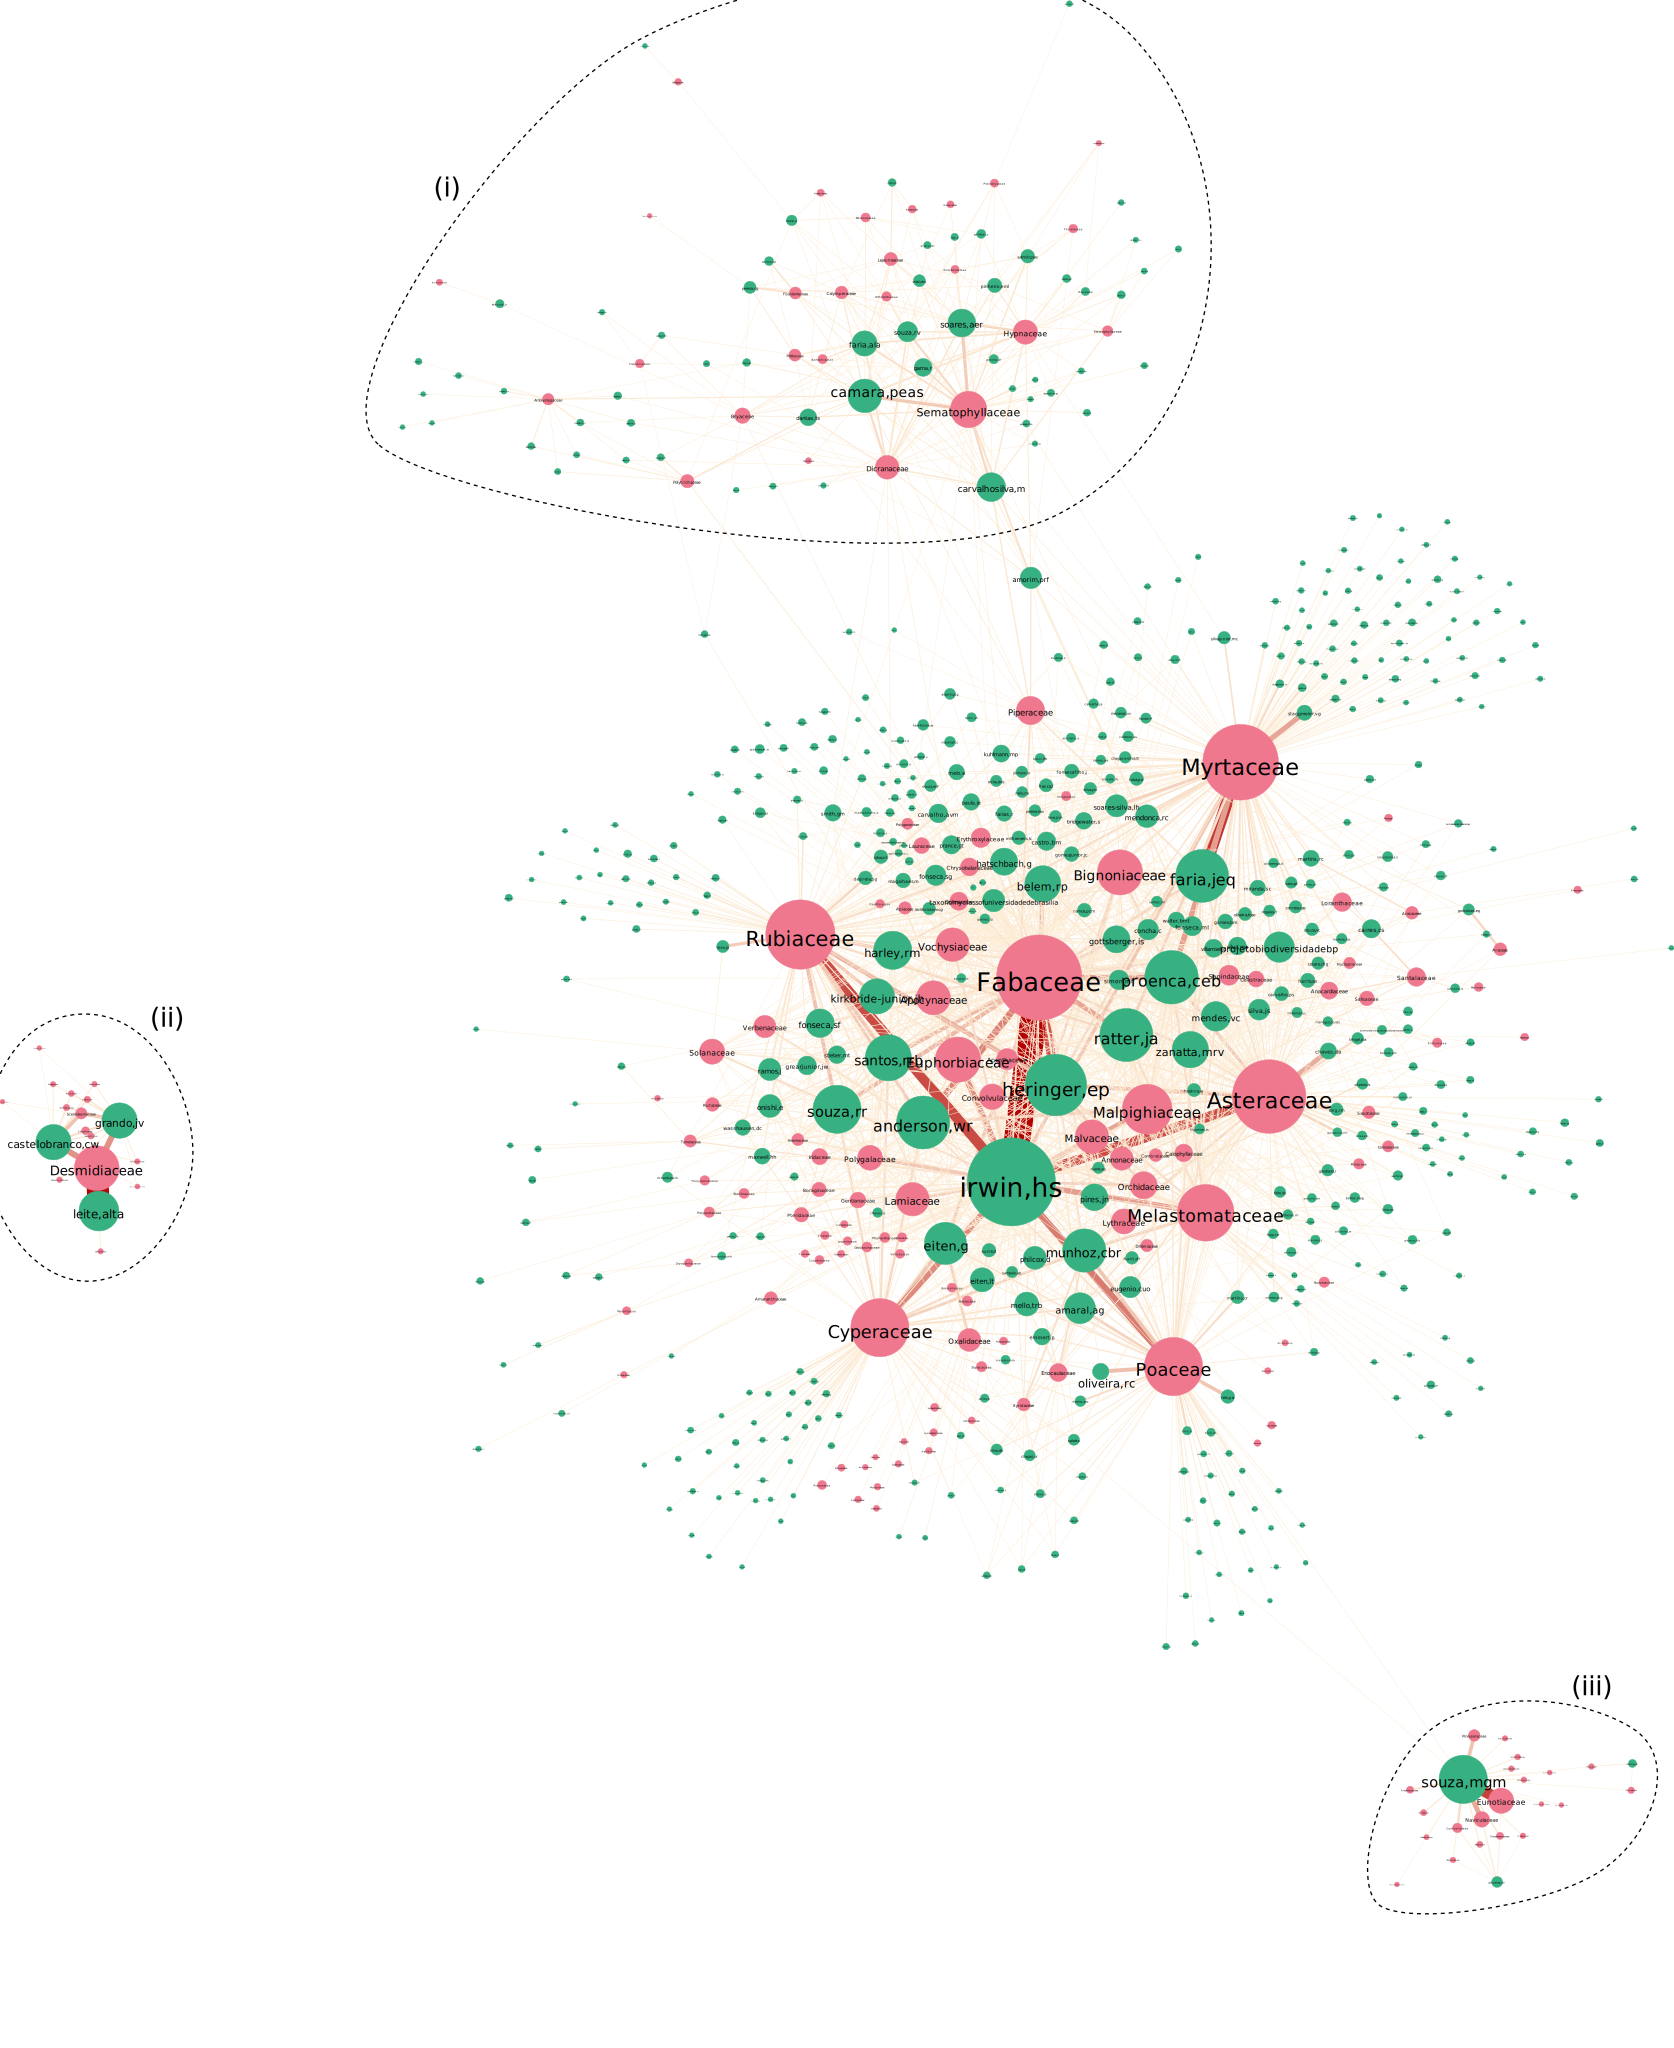
\includegraphics[width=\linewidth]{figures/casestudy_ub/scn_agg_family_general.pdf}
    \caption[alt]{ General aspect of the UB SCN network taxonomically aggregated onto the family rank. Species and collectors are respectively represented as pink and green nodes, and edges are weighted according to their \textit{count} attribute. Nodes sizing is based on their \textit{count} attribute, whilst edges color and width reflect their weight. For improving visualization we first filtered out edges with weight lower than $20$ and then omitted isolated nodes from the resulting graph. Nodes within poligons $(i)$, $(ii)$ and $(iii)$ compose visually distinguishable communities. Graph layout was computed using the \textit{ForceAtlas2} algorithm \cite{Jacomy2014}. For a better visualization experience refer to the interactive graph in the author's personal web page\footnotemark. }
    \label{fig:ub_scn_agg_family_general}
  \end{figure}
  \footnotetext{ \url{https://pedrosiracusa.github.io/networks/ub_scn_agg_family} }
}

Three communities are visually distinguishable from the central region of the network, which we'll refer to as the network core (Figure \ref{fig:ub_scn_agg_family_general}).
Although the network core could be considered a community \textit{per se}, we prefer to think of it as a region of the network that best reflects the overall interests of the majority of the most productive collectors composing the herbarium.
Nevertheless, collectors from the network core still vary considerably regarding their recording interests, as can be verified by inspecting the sets of taxa they're linked to as well as the strength of each connection. 
Those who have sampled organisms from many distinct families (and are thus considered to display a generalist collecting behavior) are placed more centrally in the network core by the layout algorithm, whereas specialists are consequently pushed towards the borders of the network core, as nearer as possible to their most recorded taxa.

\textit{Howard S. Irwin} (\textit{irwin,hs}) is the collector with most records in the network, having intensively sampled organisms from many distinct families, especially from the most central ones (illustrated in Figure \ref{fig:ub_scn_agg_family_general} as the biggest pink nodes).
The majority of his records are, in descending order, from families \textit{Fabaceae}, \textit{Rubiaceae}, \textit{Asteraceae}, \textit{Poaceae} and \textit{Cyperaceae}. 
He is also the collector holding the highest number of records for those families.
An interesting fact is that although \textit{Myrtaceae} is the second most recorded family in the UB dataset (with a total of $10951$ records), it was relatively overlooked by \textit{irwin,hs}, having himself contributed with only $399$ \textit{Myrtaceae} records. 
Instead, the main \textit{Myrtaceae} collector in the herbarium is \textit{Jair E. Faria} (\textit{faria,jeq}), who apparently has a preference towards this family, as it composes approximately $31.0\%$ of his entire records set. 
It could be insightful to investigate why a generalist collectors such as \textit{Irwin}, who mostly contributed to the herbarium in the context of the Central Brazil expedition (see Table \ref{table:ub_collectors_florescer}), was not very interested in such a predominant family from the Cerrado biome as \textit{Myrtaceae} (Figure \ref{fig:ub_scn_agg_family_general} ).
\textit{Carolyn E. B. Proença} (\textit{proenca,ceb}) is another key collector of this family, although she is also interested, to the same extent, in families \textit{Fabaceae} and \textit{Asteraceae}. 
Moreover, the figure also makes it easy to detect collectors who exclusively (or almost exclusivelly) collect each family, as it is the case of \textit{Vanessa G. Staggmeier} (\textit{staggmeier,vg}) for \textit{Myrtaceae} and \textit{Regina C. Oliveira} (\textit{oliveira,rc}) for \textit{Poaceae}.

%  TODO Communities i, ii, iii
Community $i$ represents a large part of the \textit{Cryptogams Lab}\footnote{\url{http://labcriptounb.blogspot.com.br/}} collectors team, together with the taxa they're most interested in. 
The lab is part of the University of Brasília department of botany, having \textit{Paulo Eduardo A. S. Câmara} (\textit{camara,peas}), \textit{Micheline Carvalho Silva} (\textit{carvalhosilva,m}) and \textit{Maria das Graças M. de Souza} (\textit{souza,mgm}) as the principal investigators. 
%
The first two researchers, which have been included in community $i$, are mostly interested in bryophytes (mosses and liverworts), mainly those from families \textit{Sematophyllaceae}, \textit{Hypnaceae} and \textit{Dicranaceae}.
\textit{Micheline C. Silva}, however, also shows interest towards \textit{Piperaceae}, a family of flowering plants that has also been considerably recorded by collectors from the network core. 
Therefore, \textit{Piperaceae} is an important node connecting community $i$ to the network core, as it intermediates many paths between collectors from both network regions.
%
Some PhD and MSc students from the cryptogams lab including \textit{Abel Eustáquio R. Soares} (\textit{soares,aer}), \textit{Allan Laid Alkimim Faria} (\textit{faria,ala}), \textit{Ronaldo Viveiros de Sousa} (\textit{souza,rv}), \textit{Tamara Silva Dantas} (\textit{dantas,ts}), \textit{Renato Gama} (\textit{gama,r}) and \textit{Eliana Marília Lima Pinheiro} (\textit{pinheiro,eml}) have also been placed in community $i$, and their closeness to their academic supervisor \textit{`camara,peas'} reflect their common taxonomic interests in bryophytes.

Although she is one of the principal investigators of the \textit{Cryptogams Lab}, \textit{`souza,mgm'} was placed in community $iii$ instead of $i$ due to her taxonomic interest towards algae, a taxonomic group which is overlooked by the vast majority of collectors in the herbarium, including bryophytes collectors. 
She is mostly interested in families \textit{Eunotiaceae}, \textit{Naviculaceae}, \textit{Pinnulariaceae}, which compose a group of algae known as diatoms.
There are two more collectors in community $iii$.
Together with \textit{`souza,mgm'}, \textit{Roni Ivan Rocha de Oliveira} (\textit{oliveira,rir}) was a member of a survey on the diatoms acquatic biota of the Paranã River, during years 2002 and 2003.
\textit{Drielle dos Santos Martins} (\textit{martins,ds}) was an undergraduate student and a lichen collector, having been supervised by \textit{souza,mgm}.

Another community of algae collectors is the one formed by \textit{Ana Lúcia Tostes de Aquino Leite} (\textit{leite,alta}), \textit{João Vademar Grando} \textit{grando,jv} and \textit{Christina Wyss Castelo Branco} (\textit{castelobranco,cw}) (community $ii$), which also happens to be the connected component $c_2$ itself.
\textit{Ana Lúcia Leite} has intensely collected continental green algae from family \textit{Desmidiaceae} in the Federal District while pursuing her MSc degree at the University of Brasília.
During that period she has also collected some specimens from another green algae family, \textit{Closteriaceae}, which has not been recorded by anyone else from the UB herbarium.
She is regarded as one of the UB historically relevant collectors (Table \ref{table:ub_collectors_florescer}).
%
\textit{João Grando} and \textit{Christina Castelo Branco} were also MSc students at the University of Brasília, both working under the academic supervision of Dr. \textit{Antônio José de Andrade Rocha} (not included in the UB dataset).
Besides green algae (families \textit{Desmidiaceae}, \textit{Scenedesmaceae}, \textit{Chlorellaceae} \textit{Selenastraceae} \textit{Hydrodictyaceae}), they have also collected other types of microscopic organisms, such as euglenophytes (family \textit{Euglenaceae}) and cyanobacteria (families \textit{Nostocaceae}, \textit{Oscillatoriaceae}, \textit{Chroococcaceae} and \textit{Pseudanabaenaceae}). 
All those organisms are typical of limnic systems.
 

We could use a whole set of modularity detection algorithms in order to further split the network core and identify communities which are visually less conspicuous. 
A common practice among the statistical physics community for detecting communities in bipartite networks has been to first obtain bipartite projections and then running unipartite community detection algorithms for each of them, separately.
In order to minmize information loss, obtaining weighted bipartite projections is preferred over unweighted, as the latter have shown to produce poor results \cite{Guimera2007}.


% TODO Communities in projections

\begin{figure}[!ht]
  	\centering
    \includegraphics[width=\linewidth]{figures/casestudy_ub/scn_family_projCol_communities.pdf}
    \caption{ Communities in the collectors-projection of the family-aggregated SCN in figure \ref{fig:ub_scn_agg_family_general}, in which edges with weights lower than $20$ were removed as well as isolated nodes. In order to improve visualization, communities with scores lower than $500$ were also omitted from the figure. Colors are used to distinguish communities.}
    \label{fig:ub_scn_family_projCol_communities}
\end{figure}

\begin{figure}[!ht]
  	\centering
    \includegraphics[width=\linewidth]{figures/casestudy_ub/scn_family_projSp_communities.pdf}
    \caption{ Communities in the species projection of the family-aggregated SCN in figure \ref{fig:ub_scn_agg_family_general}, in which edges with weights lower than $20$ were removed as well as isolated nodes. In order to improve visualization, communities with scores lower than $500$ were also omitted from the figure. Colors are used to distinguish communities.}
    \label{fig:ub_scn_family_projSp_communities}
\end{figure}

In order to investigate more thoroughly communities of common interests under complementary perspectives we projected the family-aggregated SCN network shown in Figure \ref{fig:ub_scn_agg_family_general} into both the collectors (Figure \ref{fig:ub_scn_family_projCol_communities}) and the species sets (Figure \ref{fig:ub_scn_family_projSp_communities}), using the approach described in section \ref{section:scn_projection}.
We used the species bag / quorum similarity rule (expression \ref{equation:cosine_similarity}) for weighting the edges in the resulting unipartite networks.


% ======================
% The Col set projection
\paragraph*{Communities in the collectors projection.}
The collectors projection of the family-aggregated UB SCN network has a total of $6768$ nodes and $5,431,799$ edges, with average node degree $\langle k \rangle = 1605$.
Although the taxonomic aggregation process does not change the number of nodes at all in a collectors projection of a SCN, the number of edges connecting collectors together increases signifficantly from lower-rank towards higher-rank aggregations, which means they also become denser.
In fact, the density of our family-aggregated SCN collectors projection is $2.37 \times 10^{-1}$, while the same projection at the species resolution is almost $10$ times sparser, with a density of $3.64 \times 10^{-2}$. 
This happens because higher-level taxa represent broader ranges of organisms, and thus assume ties from all lower-rank taxa they are composed of.
In other words the lowest the taxonomic resolution of the network model is, the most inclusive are taxa modeled as nodes, making it more likely that collectors record at least one specimen belonging to it. 

% edges filtering
We could reduce the density of the projected network by ignoring weaker ties, which form between collectors who are less similar in their species bags.
For that we define a filtering routine, which consists of iterating entries of the network's biadjacency matrix $A$ and setting elements to $0$ in case their respective values fall below a user-defined filter threshold $\phi$.
Acceptable values for the filtering coefficient $\phi$ range within the interval $[0,1[$, and represents the minimum similarity score that should be observed for a pair of collectors for their tie to be considered relevant.
Figure \ref{fig:ub_scn_projCol_filter_thresh} illustrates the effect of increasing $\phi$ on the density of the UB SCN, under three distinct taxonomic resolutions. 

\begin{figure}[!ht]
  	\centering
    \includegraphics[width=\linewidth]{figures/casestudy_ub/scn_projCol_filter_thresh.pdf}
    \caption{ This is the caption }
    \label{fig:ub_scn_projCol_filter_thresh}
\end{figure}

% We must specify some filtering threshold for ignoring less relevant ties.
% But what is a good threshold? < plot threshold vs density>
We then set $\phi = 0.8$.
This means only edges with similarity values higher than $0.8$ are kept, while weaker edges are discarded.
We also define a score metric for each connected component, by simply adding up values of the \textit{count} attributes for each member node.
For this visualization we have removed connected components with score lower than $500$.

% quickly describe the community detection algorithm used.

% Discuss some of the communities found
The collectors projection has $20$ communities, $7$ of which composing a giant component \ref{fig:ub_scn_family_projSp}.


% ======================
% The Sp set projection
% The resulting network is also very dense.
% The Sp projection is about 10 times denser than the collectors.
% Simlarly, we must define a filtering threshold
\paragraph*{Communities in the species projection.}
The species projection of the family-aggregated UB SCN network has a total of $15,344$ nodes and $19,482,923$ edges, with average node degree of $2539$.
The collectors projection has $15$ communities.








% ====================
% Assortativity in SCN
% Network resilience: If the SCN is dissortative, then it is easier to break it by removing hubs (therefore forming many specialized subgroups of collectors). Otherwise, removing any of the main hubs would not have a considerable effect on fractioning the network (Specialized communities are unlikely to be formed if an important collector leaves the herbarium). 



Communities discussed above are composed by collectors that share interests in common taxa and, conversely, taxa that has been sampled by a common set of collectors.
These are interest networks.
They do not represent collaborative ties between collectors in field.
This can be investigated with CWN models, as described below.

% ===============================
% UB Collectors Coworking Network
% -------------------------------

\subsection{The UB Collectors Coworking Network}
% TODO: Add average path size connecting collectors
% From table \ref{table:ub_collectors_florescer}, \textit{Irwin} mostly contributed to the UB herbarium from year $1962$ to $1976$, in the context of the Central Brazil Expedition carried out by the New York Botanical Garden \footnote{\url{http://sciweb.nybg.org/science2/hcol/planalto/index.asp}}. Together with \textit{William R. Anderson} (\textit{anderson,wr}), \textit{Irwin} was a key member of the expedition staff. 

As the UB was built based on the same set of records as the SCN model explored in the previous section, the number of nodes is $6768$, which is equivalent to the number of collectors nodes in the SCN.
Here all ties are established between collectors, with a total of $10391$ edges.
There are $2673$ ($39.5\%$) singleton collectors (those having no collaborations, or $k=0$).

The network is composed by a giant component, containing $3114$ nodes ($46\%$ of the nodes) and $2990$ other isolated components, holding the remaining $54\%$.
However, almost all isolated components are in fact singleton collectors (those who have never collaborated with any other collector). All singletons are considered a distinct isolated component, and that's why there are so many of them. Only $317$ isolated components are formed by collectors with at least one collaborative tie.
The percentage of nodes in the giant component is small if compared to other social networks (most are between $80\% - 90\%$) \cite{Newman}. This observed low size of the giant component might be due to records from foreign teams, which have never collected with anyone from the giant component. These records give a poor coverage of the real activities of these collectors, which could be possibly obtained from other herbaria.

The overall network density is $4.5 \times 10^{-4}$.
If we only consider the network giant component we get a density of $1.95 \times 10^{-3}$.
If we only consider the herbarium core we get a density of $x$.

\paragraph*{Distinct collaborators per collector.}
Collectors collaborate, in average, with $3.07$ distinct collectors throughout their entire careers.
However, similarly to the SCN network, degree distribution for the CWN network does not fit a poisson distribution well (which is characteristic of random networks). It fits better a power law with parameter $\alpha=2.2$.

Although team sizes are typically not very large (not exceeding 9 collaborators in the UB herbarium), some collectors have gathered a large number of collaborators throughout their carreers, much more than the average. %% TODO: Add figure with team sizes
In contrast, there are also many collectors who have never recorded collaboratively with any other collector.

Depending on the degree centrality metric we use, we get a different ranking of most influential collectors.
The non-weighted degree $k$ ranks collectors based on the total number of collaborations they've established to distinct collectors, irrespective of the number of times each association was observed.
If we use the weighted degree $k_w$ metric instead, we must specify which weighting rule to use. If we use the edge \textit{count} attribute, which is simply the number of times a given association between two collectors occur, the weighted degree for each collector is equivalent to his/her total number of collaborative records. which also considers the number of recurrent collaborations with each collaborator, we consider in the ranking rule the number of collaborative ties a collector has established to others, irrespectively of the number of distinct collectors.

We could use another weighting rule for calculating the $k_w$ centrality, for example the hyperbolic weighting.

%% TABLE HERE %%
%% FIGURE HERE %%

For a concrete example, \textit{Howard S. Irwin} (\textit{irwin,hs}) is the top collector in terms of absolute number of collaborative ties. He has collected a total of $14803$ specimens in field with others. However, the network indicates that he usually works with a more restricted team of partners. He holds only $39$ links to distinct collectors, which puts him in the $43th$ position of the rank. 
On the other hand, \textit{James A. Ratter} (\textit{ratter,ja}), who is the third with most connections to distinct collectors, is on the $20th$ position in the $k_w$ rank, with a total of $2962$ collaborative collectors.
There are only $3$ collectors in common between the top-10 collectors in the $k_w$ and the $k$ ranks.
% TODO: Include hyperbolic weighting (and compare with degree k)

As in this model it is possible for even for collaborative collectors to record some records alone, the weighted degree is not necessarily equivalent to his/her total number of records. Instead, it is equivalent to his/her total number of collaborative records.

\paragraph*{Do collaborative collectors prefer to work with other collaborative ones?}
One relevant question we might ask is whether collectors tend to form collaborative ties preferentially with others holding a similar number of collaborative ties.
Here we refer to collaborative collectors as those holding collaborative ties with many distinct collectors, irrespective of the number of times each individual link occurs. Those collectors which hold strong collaborative ties with few collaborators are thus less collaborative than the former case. In this sense, $proenca,ceb$ is considered more collaborative than $irwin,hs$, for instance.

More concretely, we want to assess whether the network is assortatively mixed.
If this is the case then we would expect to observe that most collaborators of very collaborative collectors are also very collaborative.
Conversely, collectors that do not hold many ties, for instance novice or non-collaborative experienced collectors, should preferentially connect with others with similar degrees.
This would lead to a network where highly collaborative collectors are clustered together, composing a solid core. Less collaborative ones would, instead, tend to be marginalized. % TODO: add a figure comparing those patterns

For assessing network mixing pattern we calculated the Pearson correlation coefficient $r = \frac{\sum_{xy} xy(e_{xy}-a_xb_y)}{\sigma_a \sigma_b}$ , as proposed by Newman \cite{Newman2003c} (eq. 21).
The term $e_{xy}$ represents the fraction of edges that connect nodes with degrees $x$ and $y$ in the network, such that $\sigma_{xy}e_{xy}=1$. 
Computing the correlation coefficient involves comparing the term $e_{xy}$ with the product between the percentage of all edges that start in a $x$-degree node ($a_x$) and the percentage of all edges that end in a $y$-degree node ($b_y$). The computation is carried out for each combination of degree values $x$ and $y$.
By using this metric we assess whether a correlation exists between the degrees of each pair of nodes which are connected by an edge. 
The result is bound to the $[-1,1]$ interval, where a score of $1$ indicates perfect assortativity and a score of $-1$, perfect dissortativity.
Scores close to $0$ indicate that no correlation exists between nodes, and thus the network is neither assortative nor dissortative.

For the UB collectors coworking network we obtained an assortativity score of $-0.0034$ for the network as a whole, including all the isolated components; and a score of $-0.0308$ only considering the giant component.
Both coefficients are negative and very close to zero, suggesting that collectors do collaborate with others irrespectively of their degrees. In other words, we do not observe a significant degree correlation between nodes in this network. 
This result contrasts with those from Newman's paper \cite{Newman2003b}, which shows that typically social networks display assortative mixing. Additionally states that this is one of the aspects that differentiate social networks differentiate from other types of networks. In other words, high degree nodes tend to associate to other high-degree ones. Nodes tend to associate to others of similar degree.
This is not the case for the CWN network. If we consider the network as whole, including the many isolated components, we get an assortativity coefficient of $-0.0034$, whereas if we consider only the giant component it is $-0.0308$. 
% but check {Bearman2004}... similar assortativity


% TODO: Betweeness: Which collectors facilitate collaborative behavior?
 
 
%%
%% Projected graphs info

%% If we used general graph algorithms for analyzing non-projected bipartite networks, a set of bipartite constraints would be ignored, such as only nodes from opposite sets being allowed to be adjacent. Depending on the algorithm this could be a problem or not {Borgatti2015}. Some algorithms are easily adapted to the bipartite case

%% Projections degree distribution



% Projections

% Similarity between collectors
% It should be noticed, however, that in practice collectors holding similarity values very close to one tend to be those with very few records in the dataset. More experienced collectors can have higher similarities with some collectors, but it is usually not very high.
%% PLOT max similarity vs degree


%%% QUESTIONS

%% 1. How common are collaborative recordings within the dataset?
%%% What is the proportion of collaborative records in the dataset? How many collaborators
%%% One-collector recording vs >2 collectors recordings
%%% Distribution of team size
%%% Caveats: Some collectors may not include collaborators names in the records

%% x. How likely is a novice collector to become a great collector?

%% x. Do collectors with similar interests tend to collect together?
%%% Mix of the two models
%%% Look for homophily in collectors communities, assortativity.

%% x. Which groups of species best partitionate collectors in the dataset, in terms of their collection interests? 
%%% Using SCNs
%%% Are these groups necessarily taxonomic ones (such as family)? Or could functional groups be more relevant in some cases? Or is there a geographical effect?
%%% e.g. Some group might be best classified as specialists on species inhabiting some geographical location, with some specific habit and belonging to some family rather than simply as specialists in a given family.

%% x. The Expert-location problem {Chapt. 8 of book Social Network Data Analytics}
%%% The expert team formation problem: How can we best select experts for a given job, based on how willing they are of collaborating together?
%%% Combine both SCN and CWN
\newcounter{QuestionsCounter}
\setcounter{QuestionsCounter}{1}

\subsubsection*{Question \arabic{QuestionsCounter}: What team sizes do collectors usually form?}
% Average team sizes

\stepcounter{QuestionsCounter}
\subsubsection*{Question \arabic{QuestionsCounter}: <Another question>}

\stepcounter{QuestionsCounter}
\subsubsection*{Question \arabic{QuestionsCounter}: Who are specialist/generalist collectors?}
% References {Newman2004}


% Statistical characterization of CWN structure
%% Largest component, connected components...
%% Assortativity: Do collectors with many collaborators (very collaborative) tend to associate with others that are also very collaborative?






%\subsection{Features Selection}

%% Features engineering

%\section{Model Evaluation}



\chapter{Conclusion and Perspectives}\label{conclusion_perspectives}
% ===========
% Conclusions
% -----------
In this dissertation we proposed the conceptual basis of a new approach for describing the assemblage of biological collections as a social process, driven by the taxonomic interests of contributor collectors as well as their social interactions.
We provided methods for structuring species occurrence data from biological collections into two main classes of network models, each giving distinct perspectives on the recording behavior of collectors.
\textbf{Species-Collector Networks} (SCNs) model interest relations between collectors and taxa they record, whilst \textbf{Collector CoWorking Networks} (CWNs) represent collaborative ties between collectors co-authoring specimens records. 
% UB case study
We demonstrated the use of our models by exploring the species occurrence dataset of the University of Brasília Herbarium.
Using the social network analytics framework \cite{Barbier2011,Stork2015} as a theoretical foundation, we explored structural properties of the networks, 
and investigated the formation of communities of collaboration and common interests.
We also assessed the distinctiveness of collectors regarding their taxonomic interests, their collaborativity with others, and the temporal evolution of collaborative recording in the herbarium.
Although in this study we specifically discuss SCNs and CWNs in the context of scientific biological collections, the same ideas here exposed can be also extended to other communities, such as those of nature observers (\textit{e.g.} wildlife photographers, bird watchers) and citizen scientists.


% Why structure collections data as networks?
We believe our models provide the structural basis for a more realistic understanding on how collector and taxonomic biases arise in biological collections. 
As stated by \citeonline{Marin2011}, network-based approaches allow analysts to
(\textit{i}) investigate the effects of interactions between individuals on shaping their own behaviors, rather than simply comparing static attributes of individuals within a population; and
(\textit{ii}) investigate the formation of non-homogeneous communities, composed by individuals interacting with their groups at varying levels of commitment.
We consider that these two aspects are particularly relevant in the context of biological collections.

First, collectors often start their careers being supervised by one or more collectors.
As it naturally happens in many social systems, the behavior of individuals can be strongly influenced by others at more privileged positions, and this is likely to be the case for collectors communities as well.
A network-based approach would allow us to investigate, for instance, how the collecting behavior and taxonomic interests of novice collectors are shaped by their association with more experienced ones.
Moreover, depending on its position on the network, a collector can interact with multiple groups of collectors at different extents, assuming the role of influencer in some cases while being influenced in others.
The influential power of a collector depends not only on the absolute number of connections it holds with others, but also on how strongly it intermediates other connections, how close it is to every other collector in the network, and how influential are its own connections. % Influential analysis
All these aspects can be assessed using well-known metrics (including degree, betweeness, closeness and eigenvector centralities), and could be used for investigating which collectors are most relevant for shaping the taxonomic composition of the collection. 

Second, although collectors often define their own taxonomic interests and expertises in terms of natural or functional groups of organisms, those are not necessarily the groups that best split the interests of collectors in the dataset of a given collection.
In addition, collectors (even the most specialized ones) are not restricted towards exclusively recording organisms of their expertises, nor they have uniform interest towards all of those organisms.
%
In this context, SCNs provide the structure for discovering groupings of taxa that perform better at characterizing and differentiating collectors based on their taxonomic interests (communities in the species projection); and for investigating associations of collectors to groups of taxa in a non-discrete manner, allowing collectors to be linked to taxa at multiple groups and at different intensities.
%
In fact, while some groups of taxa are more specifically recorded by distinctive communities of specialized collectors, others are recorded by a wider range of collectors, with diverse taxonomic interests.
For instance, the SCN of the UB herbarium suggests that collectors specialized in families \textit{Myrtaceae}, \textit{Poaceae} or \textit{Piperaceae} form communities of interests which are in fact more distinctive, as those families are relatively poorly recorded by collectors who are not specialists in each of them (see Figure \ref{fig:ub_scn_family_projSp_communities}).
In contrast, other families such as \textit{Fabaceae}, \textit{Melastomataceae} and \textit{Rubiaceae} are more widely recorded in the herbarium, and thus do not form a tight community of interest.


% Quality of the model
The quality of our network models strongly depends on the quality of the species occurrence dataset which is used to build them, more specifically on the fields containing the names of the collectors (\textit{recordedBy}, in TDWG standards) and the taxonomic identity of the specimen (\textit{scientificName}, in TDWG standards) of each record.
%
During this study we have explored occurrence datasets from other herbaria other than the UB, including
the RB (at the Rio de Janeiro Botanical Garden) \cite{gbif_rb}, 
the MBML (Mello Leitão Herbarium) \cite{gbif_mbml},
and the Hemilio Goeldi Museum Herbarium \cite{gbif_mpegh}.
However, we decided only to use the dataset from the UB in our case study for its relatively high quality, specifically for the two fields mentioned above.
%
In all other herbaria, the collectors field (\textit{recordedBy}) was particularly problematic.
Our hypothesis is that the low quality of this field is associated to its low value for most uses of species occurrence data, implying that not much effort has been employed by data curators towards improving its quality.
While imprecise taxonomic determinations in the \textit{scientificName} field would also lead to low quality networks, this field is critical for many other applications of occurrence data, and thus improving its quality has been extensively pursued by the biodiversity informatics community.
The most common and impacting issues associated to the collectors field are 
($i$) using inconsistent delimiter characters for separating the names of each collector in a record, leading to many non-atomized names and consequently to the existence of nodes in the network that represent more than one collector; 
($ii$) registering collectors names using inconsistent naming conventions, which makes it hard to systematically interpret what are the component parts of a name; 
($iii$) using multiple names variations for a collector, leading to collectors being represented by more than one node in the network ; and 
($iv$) only including the name of the first collector in records (and eventually aggregating all secondary collectors under the name `\textit{et. al}'), which is interpreted as an absence of collaborative ties and thus does not contribute for the formation of edges in CWNs.
Constructing the models from a low-quality dataset can therefore introduce several semantic imprecisions. 
% RecordedBy: Two classes of issues: (1) Naming inconsistencies; (2) Authorship omission


% Limitations of the model
Our models as proposed in the scope of this dissertation also have a set of limitations, which should be addressed in the future.
% The networks only reflect the view of a single institution -> joining multiple herbaria datasets
First, as the networks are built in a single step using a single dataset (which is usually provided by a single institution), they only represent a partial view of the real interests and collaborations that collectors have accumulated during their careers.
For obtaining more holistic representations, a mechanism for dynamically joining multiple occurrence datasets --- and eventually other types of data --- should be incorporated to the models.
Although one might argue that multiple datasets can be simply merged before they are passed to the constructors of the models, that would still consist of a one-step construction, requiring the availability of all data at first place.
In addition, if any other dataset were to be incorporated in the future, the model would need to be entirely reconstructed, and all necessary preprocessing routines would have to be re-executed in each one of the previous datasets.
%
We believe that the most challenging aspect of joining multiple datasets would be addressing the entity resolution problem across datasets from multiple sources. A possible solution would be to map entities in each dataset to unique identifiers (such as the ORCID\footnote{\url{https://orcid.org/}} or the id in Lattes platform\footnote{\url{http://lattes.cnpq.br/}}, the latter widely adopted by the scientific community in Brazil) using a crowdsourcing strategy, described later in this chapter.

% The geographic and temporal dimensions
Another important limitation of our models as here defined is that they are static and non-spatialized (\textit{i.e.} temporally and geographically invariant), and limited to representing relationships of a single type each.
This implies that relationships modeled in both networks are assumed to occur irrespective of temporal and geographic dimensions, which is clearly unrealistic for the phenomena they model.
As the careers of collectors have limited lifespans, they can only possibly collaborate with others if their periods of activities overlap in time.
In addition, both coworking (between collectors) and interest (involving a collector and a taxon) relationships derive from collecting events --- each happening at a determined geographic location and at some point in time ---, being thus temporally and spatially constrained.
Incorporating these two dimensions to our models is also central for capturing network evolution in their structure.
%
As in many other social systems, relationships in SCNs and CWNs change in time, as new ties are constantly formed while older ones are broken.
It is reasonable to consider that collectors interact with distinct groups of people throughout their careers, assuming distinct roles in each relationship.
For instance, we hypothesize that earlier in their careers, collectors are more likely to assume relationships and have their interests influenced by their academic supervisors or other collectors who are more experienced.
On the other hand, relationships assumed by collectors later in their careers tend to be the opposite, as they assume the role of the more experienced collector (and thus, the influencer).
Also, depending on the stage of a collector's career and the groups of collectors she interacts at that moment, we might observe substantial shifts in her taxonomic interests (while changes in her taxonomic interests can also lead to collaborating with different groups).
Other factors can also influence the patterns of recording activity of a collector, including oscillations in the availability of financial resources for field expeditions, and changes in her residence location.
% A diversity of representations for temporal networks have been proposed, which can be categorized as either lossless representations, or lossy representations \cite{Holme2015}.


% Adopting an unifying structure
% SCNs and CWNs should be stored in an unified structure, for example using the structure of multiaspect graphs (MAGs).
% MAGs allow representing edges composed of multiple features by using general graph theory, instead of tensor algebra.
% Important dimensions can be included as aspects, such as temporal and spatial, and different types of edges. 
As many applications using our models would need to combine the perspectives of both SCNs and CWNs, we also recognize the importance of adopting an unifying model for seamlessly integrating the two networks into a single structure.
Such a model should represent two types of connections (interest and coworking) and two distinct sets of nodes (collectors and species), besides incorporating the temporal and geographical dimensions into its structure.
Although the concept of \textit{multilayer networks} provides a solution for modeling dynamic complex systems with many aspects of connectivity, literature around this topic is still incipient, with many proposals though little consensus on the best way to represent them \cite{Kivela2014}.
In this context, \citeonline{Wehmuth2014} introduce the concept of \textit{Multiaspect Graphs} (MAGs), as multilayer graph abstractions that operate on the same structure as traditional directed graphs.
By using the structure of a MAG, we would represent the set of vertices, layers, time instants and geographic locations as 4 distinct \textit{aspects}; and edges as $8$-tuples, composed of pairs of elements of each aspect.
Moreover, key properties and algorithms that have been widely used for analyzing directed graphs are also extended to MAGs, which makes them a relatively simple representation for higher-order graphs.



Finally, we indicate some of the possible applications of our models.

% ============
% Applications
% ------------
\newcounter{ApplicationCase}

% Collectors Profiling and activities history
% -------------------------------------------
% Profiling collectors in terms of their activities and interests can be a way of further detecting anomalies (activity monitoring, Fawcett and Provost 1999).
% Collectors temporal, geographic and taxonomic ranges \cite{}.
% The study of collectors career trajectories cite{Borgatti2015 conclusion}.
\stepcounter{ApplicationCase}
\paragraph*{\theApplicationCase. Context inference.}
One of the main limitations of occurrence records is that they are obtained opportunistically, in a high diversity of contexts.
Even though contextual information can be associated to records (the field \textit{occurrenceRemarks}, TDWG), systematically interpreting them is complex, as it is in text format; and, moreover, this field is usually not filled.
%
The factor that leads a collector to record a specimen depends on many factors: 
the taxonomic interests and level of expertise of the collector at that time, 
the goals of the collection expedition, 
%
dataset enrichment, by associating contextual data to each occurrence record, based on information of collectors.


% Validation of collectors IDs
% ----------------------------
\stepcounter{ApplicationCase}
\paragraph*{\theApplicationCase. Crowdsourcing the validation of collectors identities.}
Given the complexity of resolving the identities of names in the collector field of occurrence datasets, one possible solution would be using a network-based \textit{collaborative validation}, in which the records validation task is distributed through many collaborators.
The general idea of the method consists of using the structure of a CWN, initially built from the non-validated dataset, for propagating a message requesting the collaboration of collectors themselves as validators.
Starting from an initial subset of influential collectors whose identities are already resolved, collectors recursively resolve the identities of as few as $5$ of their most acquainted and, in sequence, forward them the collaboration request message. % we assume collectors who collaborate in field are acquainted to each other
The process of resolving names consists of assigning unique identifiers to them, such as the ORCID or Lattes id.
Assuming that the probability that a receiver does not ignore the message depends on its esteem towards the sender, a central requirement for an efficient diffusion of the messages in the network is to start with an initial set of vertices which not only occupy central positions in the network, but which are also influential in their respective communities and, moreover, are available and willing to collaborate with the validation process.
This is analogous to studying the dynamics of contagion in network systems \cite{Gibson2005}.




% Team Formation
% --------------
\stepcounter{ApplicationCase}
\paragraph*{\theApplicationCase. Formation of teams of specialists.}
% Red lists are necessary for pointing prioritary species for conservation e.g. the Brazilian flora red list
% Besides data, it is also necessary to include a team of specialists for validating and evaluating the conservation status of species.
% We can use interest networks for systematically selecting potential collaborators
% We can use the expertise of collectors towards the areas that they have visited and the distributions of species of their expertise;
% We also can identify taxonomist specialists as those who determine the taxonomic identity of exsiccates (species-identifier networks, extending CWNs). They would best contribute as taxonomists
% Then we can select an optimal set of specialists for contributing in more specific aspects of the elaboration of lists

% Species-determiners networks
% Also model species-identifiers network, where people are linked to species they identify.
% We could additionally model networks of species and determiners, similarly to what we've present for species and collectors.
Given the diversity and complexity of life on Earth, approaching biological problems often requires the involvement of many experts in different areas.
Moreover, experts must must not be only have a substantial expertise in their respective areas, but must also be prone to collaborate.
One aspect that our models could help is in recommending the formation of teams of specialists.
The Expert team formation problem:
Given a set of requirements, the problem consists of assessing the expertise of individuals in the network (expert location problem) and recommending the formation of a team for best covering given requirement and achieving a common goal, considering how effectively they can collaborate \cite{Lappas2001}.
We can use the SCN for assessing expertises and the CWN for refining the the ranking or suggesting teams that include many collectors who have already worked together (we assume that collectors who have successfully collaborated in the past are likely to successfully collaborating in the future).
%
One application is the formation of teams of experts for big biodiversity surveys.
Coordinators of such initiatives might be interested on systems for helping choosing the most concise team to obtain the greatest diversity of experts, who have collaborated in the past.
%
One possible application is on the elaboration of red lists.
Evaluation (by the scientific community) of the conservation status of species for the elaboration of red lists (IUCN), which are important for supporting the elaboration of conservation plans, prioritizing conservation efforts.
Species are evaluated regarding their risk of becoming extinct.
The elaboration of red lists uses occurrence data intensively, and also requires the collaboration of teams of specialists, for a task-force: validating and evaluating the conservation status of species \cite{Martinelli2013}.
Species profiles are assigned to specialists.
Selecting a high number of specialists distributes the workload better, avoiding overloading specialists.
Specialists act in diverse stages of the process, since the evaluation of data quality (such as suspicious occurrences) to the evaluation of the final profiles of species of their expertise.
Specialists that are personally invited for collaborating.
During their careers, collectors develop good intuition about the communities at locations where they have been \cite{Noss1996}, which make them good validators for occurrence data.
The geographic dimension in this case is also central, as we choose teams of specialists while trying to maximize the geographical coverage recordings.
From SCN models, we could systematically obtain recommendations of specialists who are more experienced, and have most actively recorded taxonomic groups of interest.
We first evaluate their expertise
Algorithms have been proposed in literature for computing the expertise of individuals based on their positions in the network \cite{Lappas2011}








% Building Recommender Systems
% ----------------------------
\stepcounter{ApplicationCase}
\paragraph*{\theApplicationCase. Building recommender systems.}
% Sampling Site Recommendation
% Assisted planning of future biodiversity surveying is key for improving herbarium data \cite{Graham2004}.
% Strategic sampling in unsurveyed areas: identify gaps in environmental and geographic coverages \cite{Graham2004}.
% Objectivelly priorizing regions and taxa for surveys cite{Graham2004}, site selection cite{Funk2002}
% Sampling site priorization may be done based on niche models {Raxworthy}
% GDMs {Ferrier: Mapping Spatial Pattern in Biodiversity for Regional Conservation Planning: Where to from Here?}

% Collaborative filtering: The system gather information about the interest of the collectors and then proposes collectors to record new species based on the interests of others.
% Team formation support: How to optimally assemble a team of specialists who are willing to work together?
% Link prediction: Trying to predict which ties are most likely to form between entities in the network in the near future.

% Use Case: "From your collection activity pattern, you might be interested in collecting groups {} in places {}...we found a gap there. Why don't you contact team {}? They have extensively collected other groups in that location and are willing to collaborate in field. Otherwise you could contact land owner {}. His property is within that are and his renting fee is {} reais."
% < add illustration >


% Collector's productivity Score
% ------------------------------
\stepcounter{ApplicationCase}
\paragraph*{\theApplicationCase. Assessing collectors productivity.}
Pursuing careers as field naturalists are being highly discouraged within the conservation biology scientific community \cite{Noss1996}.
We currently face a shortage of researchers willing to pursue careers as field naturalists.
Their work is unappreciated by research funding agencies.
This is partially due to the high costs of field expeditions for collecting biological materials, which do not necessarily produces publishable work.
As a result, we currently face a shortage of researches exploring new areas is decreasing, and this data is critical for the construction of models.
Funding agencies must therefore incentivate the formation of new field naturalists (especially in megadiverse countries), and this can be done by incorporating metrics that value their importance as collectors.

On their duty of managing the application of public resources to scientific initiatives, research funding agencies deal with the problem of prioritizing proposals from researchers who are most capable of providing significant advance in their respective fields.
In order to assess the academic quality of researchers, agencies mainly take into account bibliometric measures including the number of papers published in high-impact journals. 
%
As the work of field naturalists require the investment of a considerable amount of time and do not necessarily revert to things that are evaluated by agencies, their work has been largely unappreciated by financing agencies.
As a consequence, we currently observe a reduction in the number of researchers who dedicate their careers to field collecting.
%
Another possible application of the network models is assigning scores to collectors based on their recording patterns, which could become produtivity metrics.
Those metrics can be used by science financing agencies, to incentivate scientists to invest in their careers as naturalists, aggregate scientific value to it.
Their metrics depends on centrality scores.
As the metrics are calculated based on published occurrence records, this would incentivate data curators towards sharing their data, supporting open science.
% Insufficient financial support for biological collections Suarez2004


% SDM
% ---
\stepcounter{ApplicationCase}
\paragraph*{\theApplicationCase. Background data selection in SDM}
% Background data selection
% Which records can we use as background data? 
% Pseudo-absences are more likely if a group of collectors potentially intereste in the species (or taxonomic group) have searched the area.
Species Distribution Modeling is one of the main uses of species occurrence data.
The goal is to correlate the occurrence of species with environmental variables.
We then project the probable distribution of species by using environmental predictors.
%
Many algorithms used in SDM are based on both presence and absence data.
Occurrence data from biological collections have been intensely used for building SDMs.
However, given the opportunistic nature of species occurrence data, the fact that a species has not been recorded at some place does not imply that they do not occur there.
True absences are not available for occurrence data.
It could simply be out of the interest of the collectors who have sampled that areas.
Pseudo-absences can be inferred. 
Some studies have selected background data based on taxonomic groups \cite{}
%
We believe that our models can be used for background data selection.
For assessing the probability that a taxon occurs in a given place, we look at the collectors who have worked near the area.
True-absence is more likely if collectors which was potentially interested in the taxon has searched the area.
Moreover, the interest of a collector towards that taxon can change depending on the time (shift in taxonomic interests), or the team ().















%------
% Ideas
% =====

% Growth forms and habits might also be a feature of preference of collectors Haripersaud2009 pg42

% Collectors behavior
% -------------------
% Collectors do not employ uniform sampling effort towards every organism included in their respective groups of interest.
%For instance, experienced collectors tend to focus on recording rare species during collecting expeditions, while overlooking others that are very common and thus assumed to be already well represented in the collection \cite{TerSteege2011}.
%In the case of plant collectors, they also show a preference towards collecting flowering and fruiting materials \cite{VanGemerden2005}.
%Defining the interests of a collector in such a way is thus imprecise, oversimplifying aspects that make taxa to assume different levels of relevance for each collector.

% Collection Centres
% ------------------
%In a study, authors have built a map of collecting density using occurrence records from the INPA herbarium, and identified regions where most of records were concentrated, which they called the collection centres \cite{Nelson1990}.

% Phylogeny and Species Bags
% --------------------------
% One issue with the species bag is that it does not incorporate phylogenetic proximity of the taxa when computing the distance of two collectors.
% It would be nice to compute collectors proximity based not only on the absolute composition of their bags but also on the phylogenetic distance of taxa themselves.
% Look at the word2vec algorithm... may be there's some perspective there..



% ---

% ----------------------------------------------------------
% Finaliza a parte no bookmark do PDF
% para que se inicie o bookmark na raiz
% e adiciona espaço de parte no Sumário
% ----------------------------------------------------------
\phantompart

% ---
% Conclusão
% ---
%\include{capitulos/conclusao}
% ---

% ----------------------------------------------------------
% ELEMENTOS PÓS-TEXTUAIS
% ----------------------------------------------------------
\postextual
% ----------------------------------------------------------

% ----------------------------------------------------------
% Referências bibliográficas
% ----------------------------------------------------------
\bibliography{bibliography}

% ----------------------------------------------------------
% Glossário
% ----------------------------------------------------------
%
% Consulte o manual da classe abntex2 para orientações sobre o glossário.
%
%\glossary

% ----------------------------------------------------------
% Apêndices
% ----------------------------------------------------------

% ---
% Inicia os apêndices
% ---
\begin{apendicesenv}

% Imprime uma página indicando o início dos apêndices
\partapendices

% Inclusão dos arquivos referentes aos apêndices
% ----------------------------------------------------------
\chapter{Collectors Ids}\label{appendix:collectors_ids}

\lipsum[50]

Names are links in the digital version of this document.
\begin{longtable}{l l}
	  id & name \\
      \hline
      amaral,ag           & \href{http://lattes.cnpq.br/0553088328180564}{Aryanne Gonçalves Amaral} \\
anderson,wr         & \hyperlink{https://plants.jstor.org/stable/10.5555/al.ap.person.bm000000177}{William Russell Anderson} \\
belem,rp            & \hyperlink{https://plants.jstor.org/stable/10.5555/al.ap.person.bm000026951}{Romeu P. Belém} \\
bridgewater,s       & \hyperlink{https://plants.jstor.org/stable/10.5555/al.ap.person.bm000120171}{Sam G. M. Bridgewater} \\
bringel,jba         & \hyperlink{http://lattes.cnpq.br/9359704960057451}{João Bernardo de Azevedo Bringel Júnior} \\
camara,peas         & \hyperlink{http://lattes.cnpq.br/2742831544064073}{Paulo Eduardo Aguiar Saraiva Câmara} \\
carvalhosilva,m     & \hyperlink{http://lattes.cnpq.br/1015868478480965}{Micheline Carvalho Silva} \\
castelobranco,cw    & \hyperlink{http://lattes.cnpq.br/6129052109183586}{Christina Wyss Castelo Branco} \\
chaves,da           & \hyperlink{http://lattes.cnpq.br/6993370381419092}{Daniel Augusto Chaves} \\
dantas,ts           & \hyperlink{http://lattes.cnpq.br/6233687711682398}{Tamara Silva Dantas} \\
eiten,g             & \hyperlink{https://plants.jstor.org/stable/10.5555/al.ap.person.bm000002352}{George Eiten} \\
eiten,lt            & \hyperlink{https://plants.jstor.org/stable/10.5555/al.ap.person.bm000002353}{Liene Teixeira Eiten} \\
eugenio,cuo         & \hyperlink{http://lattes.cnpq.br/3694741825113110}{Chesterton Ulysses Orlando Eugênio} \\
faria,ala           & \hyperlink{http://lattes.cnpq.br/3988533384771339}{Allan Laid Alkimim Faria} \\
faria,jeq           & \hyperlink{http://lattes.cnpq.br/3214384669945455}{Jair Eustáquio Quintino de Faria Júnior} \\
fonseca,sf          & \hyperlink{https://plants.jstor.org/stable/10.5555/al.ap.person.bm000117349}{Sidney F. da Fonsêca} \\
gama,r              & \hyperlink{http://lattes.cnpq.br/7699197078019809}{Renato Gama Dias Neto} \\
grando,jv           & \hyperlink{http://lattes.cnpq.br/6229685164094420}{João Vademar Grando} \\
harley,rm           & \hyperlink{https://plants.jstor.org/stable/10.5555/al.ap.person.bm000003418}{Raymond Mervyn Harley} \\
heringer,ep         & \hyperlink{https://plants.jstor.org/stable/10.5555/al.ap.person.bm000003587}{Ezechias Paulo Heringer} \\
irwin,hs            & \hyperlink{https://plants.jstor.org/stable/10.5555/al.ap.person.bm000003953}{Howard Samuel Irwin} \\
kirkbride,mcg       & \hyperlink{-}{Maria Cristina Garcia Kirkbride} \\
kirkbride-junior,jh & \hyperlink{https://plants.jstor.org/stable/10.5555/al.ap.person.bm000011449}{Joseph Harold Kirbride Jr.                        |} \\
leite,alta          & \hyperlink{http://lattes.cnpq.br/7719191749294093 }{Ana Lúcia Tostes de Aquino Leite} \\
magalhaes,m         & \hyperlink{https://plants.jstor.org/stable/10.5555/al.ap.person.bm000005315}{Geraldo Mendes Magalhães} \\
martins,ds          & \hyperlink{http://lattes.cnpq.br/5209656812635059}{Drielle dos Santos Martins} \\
mello,trb           & \hyperlink{http://lattes.cnpq.br/0930415350491316 }{Thiago de Roure Bandeira Mello} \\
munhoz,cbr          & \hyperlink{http://lattes.cnpq.br/9973242126324510}{Cássia Beatriz Rodrigues Munhoz} \\
oliveira,rc         & \hyperlink{http://lattes.cnpq.br/2968817136128886}{Regina Célia de Oliveira} \\
oliveira,rir        & \hyperlink{http://lattes.cnpq.br/7006488728244815}{Roni Ivan Rocha de Oliveira} \\
onishi,e            & \hyperlink{https://plants.jstor.org/stable/10.5555/al.ap.person.bm000053001}{Eunice Onishi} \\
pinheiro,eml        & \hyperlink{http://lattes.cnpq.br/7238835279276067}{Eliana Marília Lima Pinheiro} \\
pires,jn            & \hyperlink{https://plants.jstor.org/stable/10.5555/al.ap.person.bm000006559}{João Murça Pires} \\
proenca,ceb         & \hyperlink{http://lattes.cnpq.br/8243382046974477}{Carolyn Elinores Barnes Proença} \\
ratter,ja           & \hyperlink{https://plants.jstor.org/stable/10.5555/al.ap.person.bm000023562}{James Alexander Ratter} \\
santos,rrb          & \hyperlink{https://plants.jstor.org/stable/10.5555/al.ap.person.bm000032907}{Raimundo Reis dos Santos} \\
soares,aer          & \hyperlink{http://lattes.cnpq.br/4908757546415140}{Abel Eustáquio Rocha Soares} \\
souza,mgm           & \hyperlink{http://lattes.cnpq.br/2817470874123772}{Maria das Graças Machado de Souza} \\
souza,rr            & \hyperlink{https://plants.jstor.org/stable/10.5555/al.ap.person.bm000055998 }{Raimundo Souza} \\
souza,rv            & \hyperlink{http://lattes.cnpq.br/2008471425847512}{Ronaldo Viveiros de Sousa} \\
staggmeyer,vg       & \hyperlink{http://lattes.cnpq.br/4357034543526737}{Vanessa Graziele Staggemeier} \\
stieber,mt          & \hyperlink{https://plants.jstor.org/stable/10.5555/al.ap.person.bm000010969}{Michael Thomas Stieber} \\
zanatta,mrv         & \hyperlink{http://lattes.cnpq.br/5981278331253704}{Maria Rosa Vargas Zanatta} \\
      \hline
\end{longtable}
%\include{apendices/apendiceB}
%\include{apendices/apendiceC}
% ----------------------------------------------------------

\end{apendicesenv}
% ---

% ----------------------------------------------------------
% Anexos
% ----------------------------------------------------------

% ---
% Inicia os anexos
% ---
\begin{anexosenv}

% Imprime uma página indicando o início dos anexos
\partanexos

% Inclusão dos arquivos referentes aos anexos
% ----------------------------------------------------------
%\include{anexos/anexoA}
%\include{anexos/anexoB}
%\include{anexos/anexoC}
% ----------------------------------------------------------

\end{anexosenv}

%---------------------------------------------------------------------
% INDICE REMISSIVO
%---------------------------------------------------------------------
\phantompart
\printindex
%---------------------------------------------------------------------

\end{document}
